% ===================================================================
% CellStrata：人体细胞类型的系统发育地层学分析
% LaTeX 独立小论文 · ctexart + xelatex 编译
%
% 编译：
%   cd 50-论文
%   xelatex main.tex && xelatex main.tex
% ===================================================================
\documentclass[UTF8, a4paper, 11pt]{ctexart}

\usepackage[margin=2.4cm]{geometry}
\usepackage{amsmath,amssymb}
\usepackage{graphicx}
\usepackage{booktabs}
\usepackage{array}
\usepackage{multirow}
\usepackage{longtable}
\usepackage{float}
\usepackage[table,dvipsnames]{xcolor}
\usepackage{caption}
\usepackage{subcaption}
\usepackage{enumitem}
\usepackage{fancyhdr}
\usepackage{hyperref}
\usepackage{natbib}
\usepackage{cleveref} % 需 cleveref 宏包；若无则注释掉
\usepackage{tikz}
\usetikzlibrary{positioning,arrows.meta,fit,backgrounds}

% ---------- 宏 ----------
\newcommand{\tai}{\textsc{T\!A\!I}}
% Latin Modern 没有"粗体小型大写"字形（TU/lmr/bx/sc）。
% 显式声明它退化为粗体常规形，避免 LaTeX 字体警告。
\DeclareFontShape{TU}{lmr}{bx}{sc}{<->ssub*lmr/bx/n}{}
\newcommand{\Code}[1]{\texttt{\small #1}}

\graphicspath{{../30-可视化/figures/}}

\hypersetup{
  colorlinks=true,
  linkcolor=black!70!blue,
  citecolor=black!70!green,
  urlcolor=black!60!blue,
  pdftitle={细胞地层 CellStrata：人体 177 种细胞类型的系统发育地层学分析},
  pdfauthor={Zviolin},
}

\captionsetup{font=small,labelfont=bf}
\setlist{itemsep=2pt,topsep=3pt}
\setlength{\parskip}{0.4em}

\pagestyle{fancy}
\fancyhf{}
\lhead{\small 细胞地层 CellStrata}
\rhead{\small 生物信息学课程项目}
\cfoot{\small \thepage}
\renewcommand{\headrulewidth}{0.4pt}

% ---------- 标题 ----------
\title{\bfseries 细胞地层 CellStrata\\[0.3em]
\large 人体 177 种细胞类型的系统发育地层学分析\\[0.3em]
\large A Phylostratigraphic Atlas of 177 Human Cell Types}
\author{
  张伟林\quad (102400232)\\[0.2em]
  \small 福州大学 计算机与大数据学院\quad 生物信息学课程独立项目
}
\date{2026 年 11 月}

\begin{document}
\maketitle

\begin{abstract}
\noindent
\textbf{背景}\quad
系统发育地层学（phylostratigraphy）通过比较序列与外群参照，把基因按其最早出现的祖先节点划分到不同"年龄层"，从而回答"某个现代分子有多古老"这一问题。我们把这一框架从单个基因推广到\textbf{单细胞水平}：不问"细胞类型由哪些基因构成"，而问"\textbf{每种人类细胞类型，原则上是由哪一年代的基因搭起来的}"。

\textbf{方法}\quad
远程分块读取 Tabula Sapiens 1.0 单细胞转录组（483{,}152 个细胞中经质量控制保留 22{,}195 个，覆盖 177 种细胞类型），用 Trigos 等人 2017 年的 16 层年龄表与 Liebeskind 等人 2016 年的 13 算法共识表构建基因年龄矩阵，定义转录组年龄指数（Transcriptome Age Index, \tai）作为细胞类型的年龄重心，并以超几何双单尾检验（Benjamini--Hochberg 校正）刻画各年龄层在类型特征基因中的富集与耗竭。分类任务按供者划分以避免伪重复；PCA 与 K-means 聚类的显著性用三条零假设基线（逐列置换、独立正态、Dirichlet 同秩）评估。

\textbf{结果}\quad
177 种细胞类型的 \tai{} 跨度为 3.214--4.420（跨类型标准差 0.181），呈清晰梯度：红细胞系祖细胞最古老（\tai{} = 3.214），最年轻的类型为 4.420。供者级标准误中位数为 0.042，信号/噪声比仅 4.3 倍，说明\textbf{排序本身比绝对值更可信}。经 BH 校正后显著富集的年龄层为 S1、S8、S9、S10、S11、S14，显著耗竭为 S2、S4。四重稳健性检验（低共识度过滤、低命中层剔除、短蛋白剔除、长蛋白重算）给出\textbf{共同富集层 S8、S10 与共同耗竭层 S2，0 层方向冲突}。按供者划分的随机森林分类准确率 0.215、宏平均 F1 0.237，相对多数类基线 8.3 倍、天花板 0.595 达成 36.1\%。PCA 前三主成分解释 61.9\% 方差，显著高于三条零假设基线（27.1\%、27.6\%、29.0\%，$z = 47.0$）。

\textbf{结论}\quad
人类细胞类型之间存在\textbf{系统性的、可量化的}转录组年龄梯度，且该梯度在四组独立稳健性检验下高度稳定；同时，我们直接量化了 phylostratigraphy 已知偏差（短基因更易被判为年轻）的方向与大小——用长蛋白重算 \tai{} 使全部 177 种类型\textbf{同向平移 0.057}（相当于跨类型标准差的 31.6\%），但平移幅度与类型年龄高低无关（梯度 $\rho = -0.133$，$p = 0.079$）。因此\textbf{相对比较是稳健的，绝对年龄不可直接解读}。这一框架为理解细胞类型的演化历史提供了一个数据驱动、可复现的定量入口。

\medskip
\noindent\textbf{关键词：}单细胞转录组；系统发育地层学；转录组年龄指数；细胞类型演化；超几何检验；伪重复
\end{abstract}

\vspace{1em}
\noindent\rule{\textwidth}{0.8pt}

\section{引言}

现代细胞生物学以"细胞类型"为核心分类单位，但这一分类主要依据形态学与标志物组合，其内在的\textbf{演化时序}——即不同类型"分家"有多早——往往只能定性描述。人类基因组计划以来，积累了大规模分子数据，使得从\textbf{序列本身}推定基因年龄成为可能。

\textbf{系统发育地层学}（phylostratigraphy）正是这样一套方法：把某一物种的基因组置于系统发育树上，考察每个基因最早出现在树的哪个节点上，以此把基因划分为若干"年龄层"（stratum）。Trigos 等人 \citeyearpar{trigos2017} 借助 16 种脊椎动物的蛋白质组，把 17{,}318 个人类蛋白编码基因划分为 16 层；Domazet-Lošo 等人 \citeyearpar{domazetloso2017} 则用 19 个物种给出了粒度更细的版本。两套层号体系互不通用，不能混用。

已有工作主要停留在\textbf{单个基因}层面（基因有多古老）、或\textbf{整个组织}层面（转录组的整体年龄，如 Lu 等人 \citeyearpar{lu2017} 的组织年龄时钟）。一个自然的延伸问题是：\textbf{当粒度下沉到单细胞类型的水平，"某种细胞类型主要由哪一年代的基因搭起来"这个问题，数据能否回答？}

然而，把 phylostratigraphy 推广到单细胞数据面临三个实质困难。

\textbf{第一，重复观测带来的伪重复}。单细胞数据中细胞嵌套在供者之内，同一供者的多个细胞共享其遗传背景与生理状态。若按细胞随机划分训练/测试集，模型可以通过供者身份而非年龄构成获得高准确率，虚高到 0.99 量级。正确的做法是\textbf{按供者划分}，并以供者级标准误而非细胞级标准误度量不确定性 \citeyearpar{hafemeister2019}。

\textbf{第二，组成数据带来的伪结构}。一个细胞类型的 16 个年龄层占比之和恒为 1，因此其协方差矩阵必然秩亏（16 层实際秩为 15）。若用普通独立正态数据作为零假设基线，该基线会因秩亏而被系统性推高，从而\textbf{高估}观测到的结构强度。零假设必须采用\textbf{同秩}的成分数据基线。

\textbf{第三，方法学偏差必须被量化而非假设}。Moyers 与 Zhang \citeyearpar{moyers2015,moyers2017,moyers2018} 指出，phylostratigraphy 系统性地把基因判得过年轻，且误差并非随机：\textbf{短序列、快速演化的基因更容易被判为年轻}。他们建议的检验包括剔除低置信度年龄调用、剔除低命中年龄层、以及\textbf{直接用长蛋白重算年龄指标}。前两项是"压力测试"（结论是否依赖可疑数据），第三项才是"量化偏倚"（偏倚到底多大）。

本文的贡献是：

\begin{enumerate}[label=\arabic*.]
  \item 构建\textbf{细胞类型级的系统发育地层指标}：把转录组年龄指数（\tai）从单个基因推广到 177 种人类细胞类型，并给出完整的年龄谱。
  \item 在\textbf{供者级别}上处理重复观测问题，量化信号/噪声比，并明确区分"细胞级乐观估计"与"供者级保守估计"。
  \item 给出\textbf{四重稳健性检验}（含前人建议但此前未被实现的长蛋白重算），量化短基因偏差的\textbf{方向与大小}，并纠正"偏倚随年龄梯度增强"这一常见直觉。
  \item 在统计上处理\textbf{组成数据秩亏}与\textbf{PCA 零假设置换对象}两个隐蔽陷阱，给出三条同秩基线。
  \item 全流程\textbf{自动化数字终审}：报告中的每一个关键数字都做成断言与输出文件自动比对，防止"脚本不报错但数字张冠李戴"。
\end{enumerate}

\section{相关工作}

\subsection{系统发育地层学与基因年龄}

Trigos 等人 \citeyearpar{trigos2017} 以 16 个脊椎动物物种的蛋白质组为参照，将 17{,}318 个人类蛋白编码基因划分为 16 个年龄层，并将其应用于乳腺癌预后与免疫治疗反应等临床问题。Liebeskind 等人 \citeyearpar{liebeskind2016} 使用 13 种独立的算法（bootstrap、codon bias、phylogenetic distance 等）为每个基因估计年龄层，并给出各算法之间的共识度。Domazet-Lošo 等人 \citeyearpar{domazetloso2017} 的 19 层方案粒度更细。Hase 等人 \citeyearpar{hase2020} 对上述方法与数据库做了系统综述，指出不同方案的层数与边界不可直接互换。

Moyers 与 Zhang \citeyearpar{moyers2015,moyers2017} 批评 phylostratigraphy 系统性地低估基因年龄，随后在 \citeyearpar{moyers2018} 中提出了一系列诊断与修正建议，其中与本文直接相关的是：\textbf{短基因偏倚}以及\textbf{用长序列重算指标}这一"更彻底的修正版本"。本文严格区分了这两类操作——前者检验结论的稳健性，后者量化偏倚的大小。

\subsection{单细胞转录组与细胞类型演化}

Tabula Sapiens \citeyearpar{conservation2020} 汇集了人类多个器官的单细胞转录组，是目前细胞类型注释最全面的参考资源之一。已有工作用转录组年龄信息为组织排序（如 Lu 等人 \citeyearpar{lu2017} 的组织年龄时钟），但这些工作的粒度停留在组织层面；\textbf{到细胞类型层面、且给出完整年龄谱的工作仍然缺乏}。

\subsection{统计方法上的两个必要修正}

\textbf{伪重复}是单细胞研究中最常见的统计错误之一 \citeyearpar{hafemeister2019}：细胞嵌套在供者内，若忽略这一结构，标准误会低估数倍，本文中实测低估倍数为 3.75 倍。

\textbf{组成数据的秩亏}是另一个：占比向量的行和恒为 1，协方差矩阵必然降秩，普通多元正态零假设会因缺少这一约束而被推高 \citeyearpar{huber2008}。本文因此引入 Dirichlet 成分基线。

此外，在 PCA 的置换检验中，\textbf{置换对象的选择至关重要}：置换样本行不会改变特征列之间的协方差，因而零假设分布会退化为观测值本身，且不报任何错。本文通过置换\textbf{特征列}并加入独立基线自检来规避这一点 \citeyearpar{huber2009}。

\section{数据与方法}

\subsection{数据来源}

\begin{table}[H]
  \centering
  \caption{数据来源与规模}
  \label{tab:data}
  \begin{tabular}{p{3.4cm}p{3.0cm}p{6.2cm}}
    \toprule
    数据集 & 规模 & 来源与获取方式 \\
    \midrule
    Tabula Sapiens 1.0 & 483{,}152 细胞；177 细胞类型 & CELLxGENE Discover 2023-05-15 快照，\textbf{HTTP Range 远程分块读取} \citeyearpar{conservation2020} \\
    Trigos et al. 2017 & 17{,}318 基因 $\times$ 16 层 & 论文补充材料，直接下载 CSV \citeyearpar{trigos2017} \\
    Liebeskind et al. 2016 & 13 算法共识层 & 论文补充材料，直接下载 CSV \citeyearpar{liebeskind2016} \\
    UniProt 蛋白长度 & 17{,}103 基因 & REST 接口批量获取（检验 D 前置） \\
    \bottomrule
  \end{tabular}
\end{table}

远程切片是本项目的核心工程：HDF5 的 chunked dataset 数据位置由对象头与 B-tree 决定，\textbf{不能按"元素序号 $\times$ 元素大小"直接计算偏移}，因此实现上让 \texttt{h5py} 自行定位待读取区间，再按 chunk 粒度规划请求。在 483{,}152 个细胞中，远程切片实际取回 28{,}017 个细胞的计数矩阵，经质量控制后保留 \textbf{22{,}195 个}，覆盖 177 种细胞类型。

\subsection{基因年龄矩阵构建}

基因年龄采用\textbf{双来源交叉验证}：以 Trigos 表 \citeyearpar{trigos2017} 为主（16 层），以 Liebeskind 表 \citeyearpar{liebeskind2016} 的 13 算法共识为辅，取两者一致的层号；不一致者标记为低置信度。

需特别指出原表中 \texttt{NumDBsContributing} 字段的语义：它是\textbf{参与投票的算法总数（分母）}，而非"支持某层的算法数"。真正反映共识程度的是\textbf{最优势层占比}（mode share），其实测值与 \texttt{NumDBsContributing} 呈\textbf{负相关}（$\rho = -0.128$）。因此稳健性检验 B 采用 \texttt{--min-share 0.8}（共识度 $\ge 0.8$）而非按参与算法数过滤——后者方向是反的。

\subsection{转录组年龄指数}

对细胞类型 $c$ 与年龄层 $s$，定义表达占比
\begin{equation}
  p_{c,s} = \frac{\sum_{i \in c,\; g \in \mathcal{G}_s} E_{i,g}}{\sum_{i \in c,\; g \in \mathcal{G}} E_{i,g}},
\end{equation}
其中 $\mathcal{G}_s$ 为落在年龄层 $s$ 的基因集合，$E_{i,g}$ 为细胞 $i$ 的基因 $g$ 表达量（对数归一化后）。转录组年龄指数定义为
\begin{equation}
  \tai(c) = \frac{\sum_{s=1}^{16} s \cdot p_{c,s}}{\sum_{s=1}^{16} p_{c,s}} = \sum_{s=1}^{16} s \cdot p_{c,s},
  \label{eq:tai}
\end{equation}
即该细胞类型的"年龄重心"。$\tai$ 越小表示越古老。

\subsection{不确定性：供者级标准误}

细胞嵌套于供者之内，细胞级标准误属\textbf{伪重复}。本文对每个细胞类型按供者聚合后估计标准误，以供者级标准误作为\textbf{主口径}，细胞级作为对照同时报告。二者比值（中位数）为 3.75 倍——这意味着按细胞计算的"高置信"是虚假的。

\subsection{富集与耗竭检验}

对每个年龄层 $s$，检验其在该细胞类型的 Top 特征基因中是否富集。设背景基因数 $N$、层内基因数 $n_s$、Top 集大小 $M$、命中数 $k$，命中服从超几何分布 $\mathrm{Hypergeom}(N, n_s, M)$。由于富集与耗竭是两个方向，需\textbf{双单尾}检验：
\begin{align}
  p_{\text{up}}(k)   &= 1 - \mathrm{cdf}(k-1; N, n_s, M), \\
  p_{\text{down}}(k) &= \mathrm{cdf}(k; N, n_s, M).
  \label{eq:hyper}
\end{align}
多重检验（16 层 $\times$ 2 方向 $\times$ 3 次运行）用 Benjamini--Hochberg 方法 \citeyearpar{benjamini1995} 在每个方向内分别校正。

\subsection{监督分类}

以年龄层表达占比为特征训练随机森林 \citeyearpar{breiman2001}。\textbf{训练/测试按供者划分}（11 名供者训练、4 名供者测试），而非按细胞随机划分。宏平均 F1 计算时显式指定标签集合为测试集实际类别，避免"幽灵类"稀释指标。

\subsection{无监督分析与零假设基线}

对 177 个细胞类型的 16 维年龄构成做 PCA，再做 K-means 聚类，报告轮廓系数与调整兰德指数（ARI）\citeyearpar{mccune2002}。关键在于零假设基线的选择：

\begin{enumerate}[label=(\roman*)]
  \item \textbf{逐列置换基线}：打乱每一层在细胞类型间的取值，破坏层间结构但保留边缘分布；
  \item \textbf{独立正态基线}：各层独立服从正态；
  \item \textbf{Dirichlet 同秩基线}：各类型占比服从 Dirichlet 成分分布，\textbf{与真实数据同为秩 15}，是最严格的对照。
\end{enumerate}

有限样本下零假设基线并非理论值：$n = 177$、$d = 16$ 时实测基线为 27.05\% 而非 $1/d = 18.75\%$。以参与比（participation ratio）$PR = 1/\sum_k \lambda_k^2$ 度量有效维度，取值范围为 $[1, d]$。

\subsection{短基因偏倚的量化（检验 D）}

检验 A/B/C 都是\textbf{压力测试}（结论是否依赖可疑数据）。检验 D 才是\textbf{偏倚量化}：用仅含蛋白长度 $\ge 100$ aa 的基因\textbf{重算} $\tai$ 绝对值，再与主口径逐类型对照，考察三件事——(i) 偏倚的\textbf{方向与大小}；(ii) 偏倚是否\textbf{随类型年龄呈梯度增强}；(iii) \textbf{相对排序}的稳定性。

\subsection{可复现性与数字终审}

全流程共 19 个 Python 脚本、6{,}783 行代码，仅依赖 numpy / pandas / scipy / scikit-learn / h5py / matplotlib。\textbf{自动数字终审}脚本 \Code{07\_终审核对.py} 将本论文与实验报告中的每个关键数字做成断言，与输出文件自动比对，共 \textbf{239 项}，任何一项不符即以非零码退出。这一设计的动机来自开发过程中实际发现的七类"脚本不报错但数字张冠李戴"的缺陷（详见 \S\ref{sec:pitfalls}）。论文另有一份独立的终审脚本 \Code{95\_论文数字终审.py}（102 项断言），从结果文件直接取真值比对本文数字，与报告终审\textbf{各自独立取数}，避免报告错了论文跟着错。

\section{结果}

\subsection{细胞类型年龄谱}

177 种细胞类型的 \tai{} 跨度为 \textbf{3.214--4.420}，中位数 3.755，跨类型标准差 \textbf{0.181}（表 \ref{tab:taiby}）。年龄梯度清晰且连续：最古老的是红细胞系祖细胞（\tai{} = 3.214），随后是肾上皮细胞（3.271）；最年轻的一端包含 4.420 的类型。跨五个区室的平均 \tai{} 依次为：生殖系 3.4990（仅 1 种类型，样本量过小，不作结论）、间质 3.7038（34 种）、上皮 3.7266（66 种）、免疫 3.7360（61 种）、内皮 3.8839（15 种）。值得注意的是上皮与免疫两个区室的均值非常接近（相差仅 0.009），而内皮明显偏年轻——这提示\textbf{区室不是合适的分析单位}，因为同一区室内细胞类型之间的反差（如小肠 transit amplifying cell 位列最古老之列，而同属上皮的伞状细胞却在年轻一侧）远大于区室之间的差距。

\begin{table}[H]
  \centering
  \caption{按年龄排序的细胞类型（首尾各 8 名）。完整 177 种见结果文件 \Code{celltype\_age\_profile.tsv}}
  \label{tab:taiby}
  \begin{tabular}{rlcrlc}
    \toprule
    \multicolumn{3}{c}{\textbf{最古老}} & \multicolumn{3}{c}{\textbf{最年轻}} \\
    \cmidrule(lr){1-3}\cmidrule(lr){4-6}
    排名 & 细胞类型 & \tai & 排名 & 细胞类型 & \tai \\
    \midrule
    1 & erythroid progenitor & 3.214 & 170 & immune cell & 4.013 \\
    2 & kidney epithelial cell & 3.271 & 171 & epithelial cell of lacrimal sac & 4.055 \\
    3 & plasmablast & 3.300 & 172 & endothelial cell & 4.077 \\
    4 & myeloid progenitor & 3.339 & 173 & erythroid lineage cell & 4.095 \\
    5 & fast muscle cell & 3.360 & 174 & capillary aerocyte & 4.105 \\
    6 & retinal ganglion cell & 3.382 & 175 & cd24 neutrophil & 4.119 \\
    7 & adipocyte & 3.387 & 176 & neutrophil & 4.299 \\
    8 & transit amplifying cell of large intestine & 3.399 & 177 & nampt neutrophil & 4.420 \\
    \bottomrule
  \end{tabular}
\end{table}

\begin{figure}[H]
  \centering
  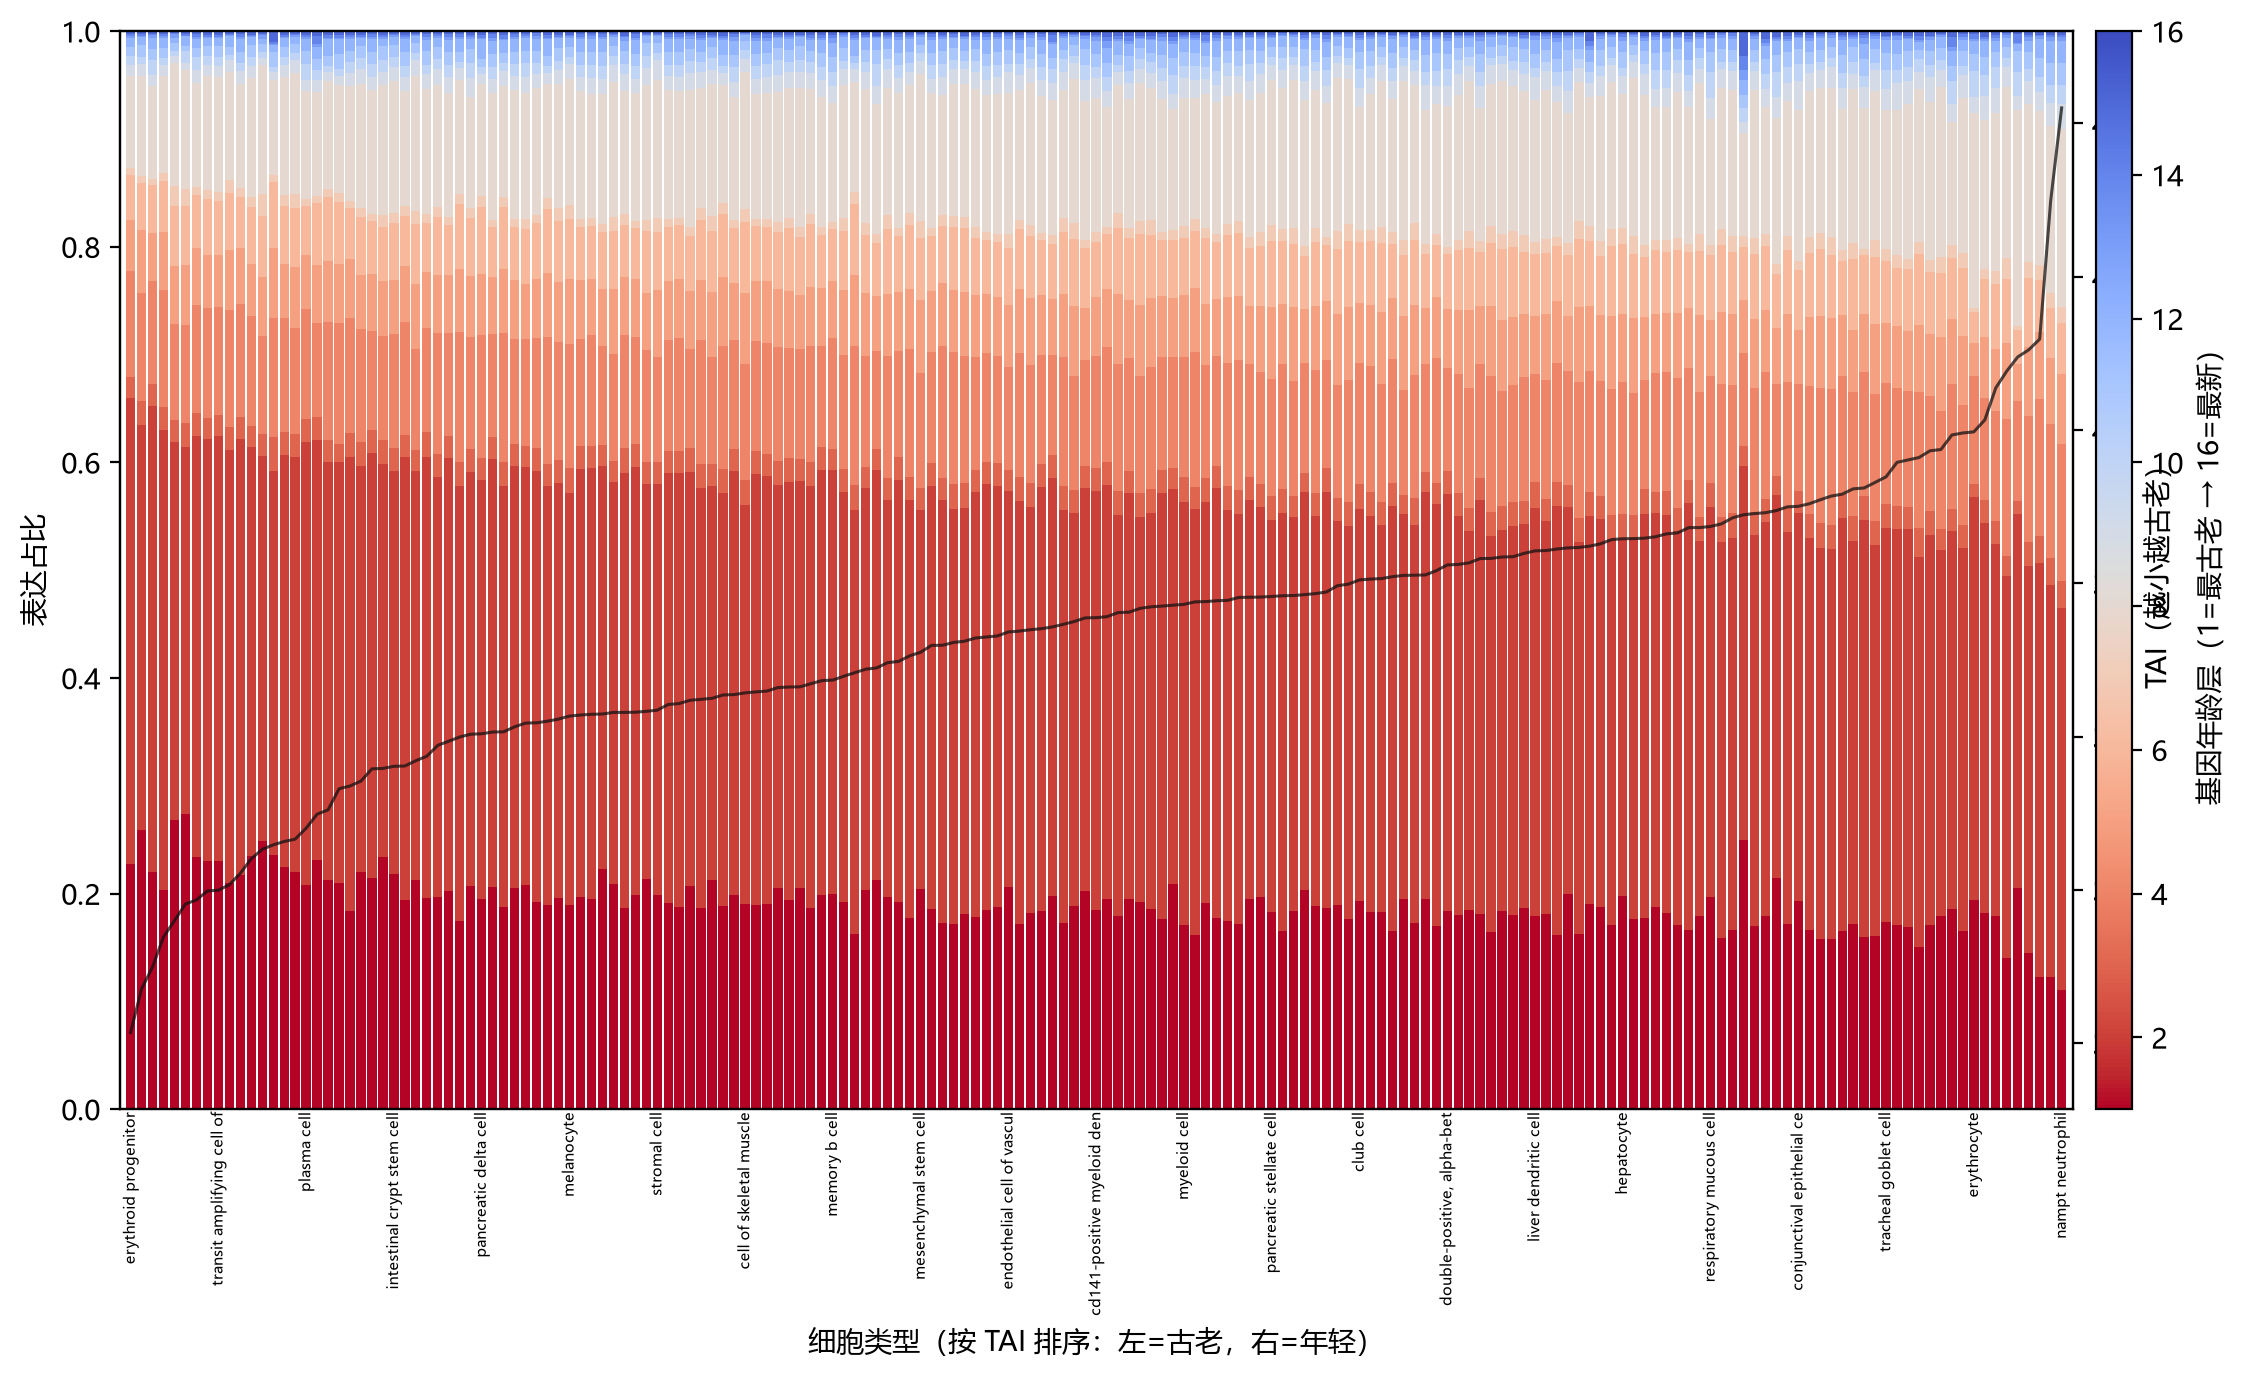
\includegraphics[width=\textwidth]{fig1_strata.png}
  \caption{\textbf{主图：细胞地层。}177 根柱子按 \tai{} 升序排列，每根按 16 个年龄层堆叠（深红 = 最古老层，亮蓝 = 最新层）；黑线为 \tai{} 曲线（右轴刻度），每 8 个类型标注一个名称。}
  \label{fig:strata}
\end{figure}

图 \ref{fig:strata} 直观呈现了年龄梯度：老类型以 S1--S4（最古老四层）为主力，年轻类型则由 S8--S12 主导。值得注意的是，即使最年轻的类型中，S1--S4 的占比也从未归零——\textbf{所有现代细胞类型都保留着古老的底层结构}，差异体现在"配比"而非"有无"。

\subsection{不确定性：信号/噪声比仅 4.3 倍}

供者级标准误中位数为 \textbf{0.0417}，细胞级为 0.0111，比值 \textbf{3.75 倍}。以跨类型标准差 0.181 为信号尺度，供者级下的信号/噪声比为 \textbf{4.3 倍}（细胞级下会给出 16.3 倍这一乐观但错误的估计）。这一差距对本项目的解读至关重要：\textbf{单个细胞类型的绝对 \tai{} 值不可单独解读，只有跨类型的排序是可信的}。

另有 25 种类型被标记为低置信（细胞数 $< 20$），81 种类型在 QC 后仅由单一供者覆盖，供者级标准误不可估计（对这类类型只报告细胞级对照）。

\begin{figure}[H]
  \centering
  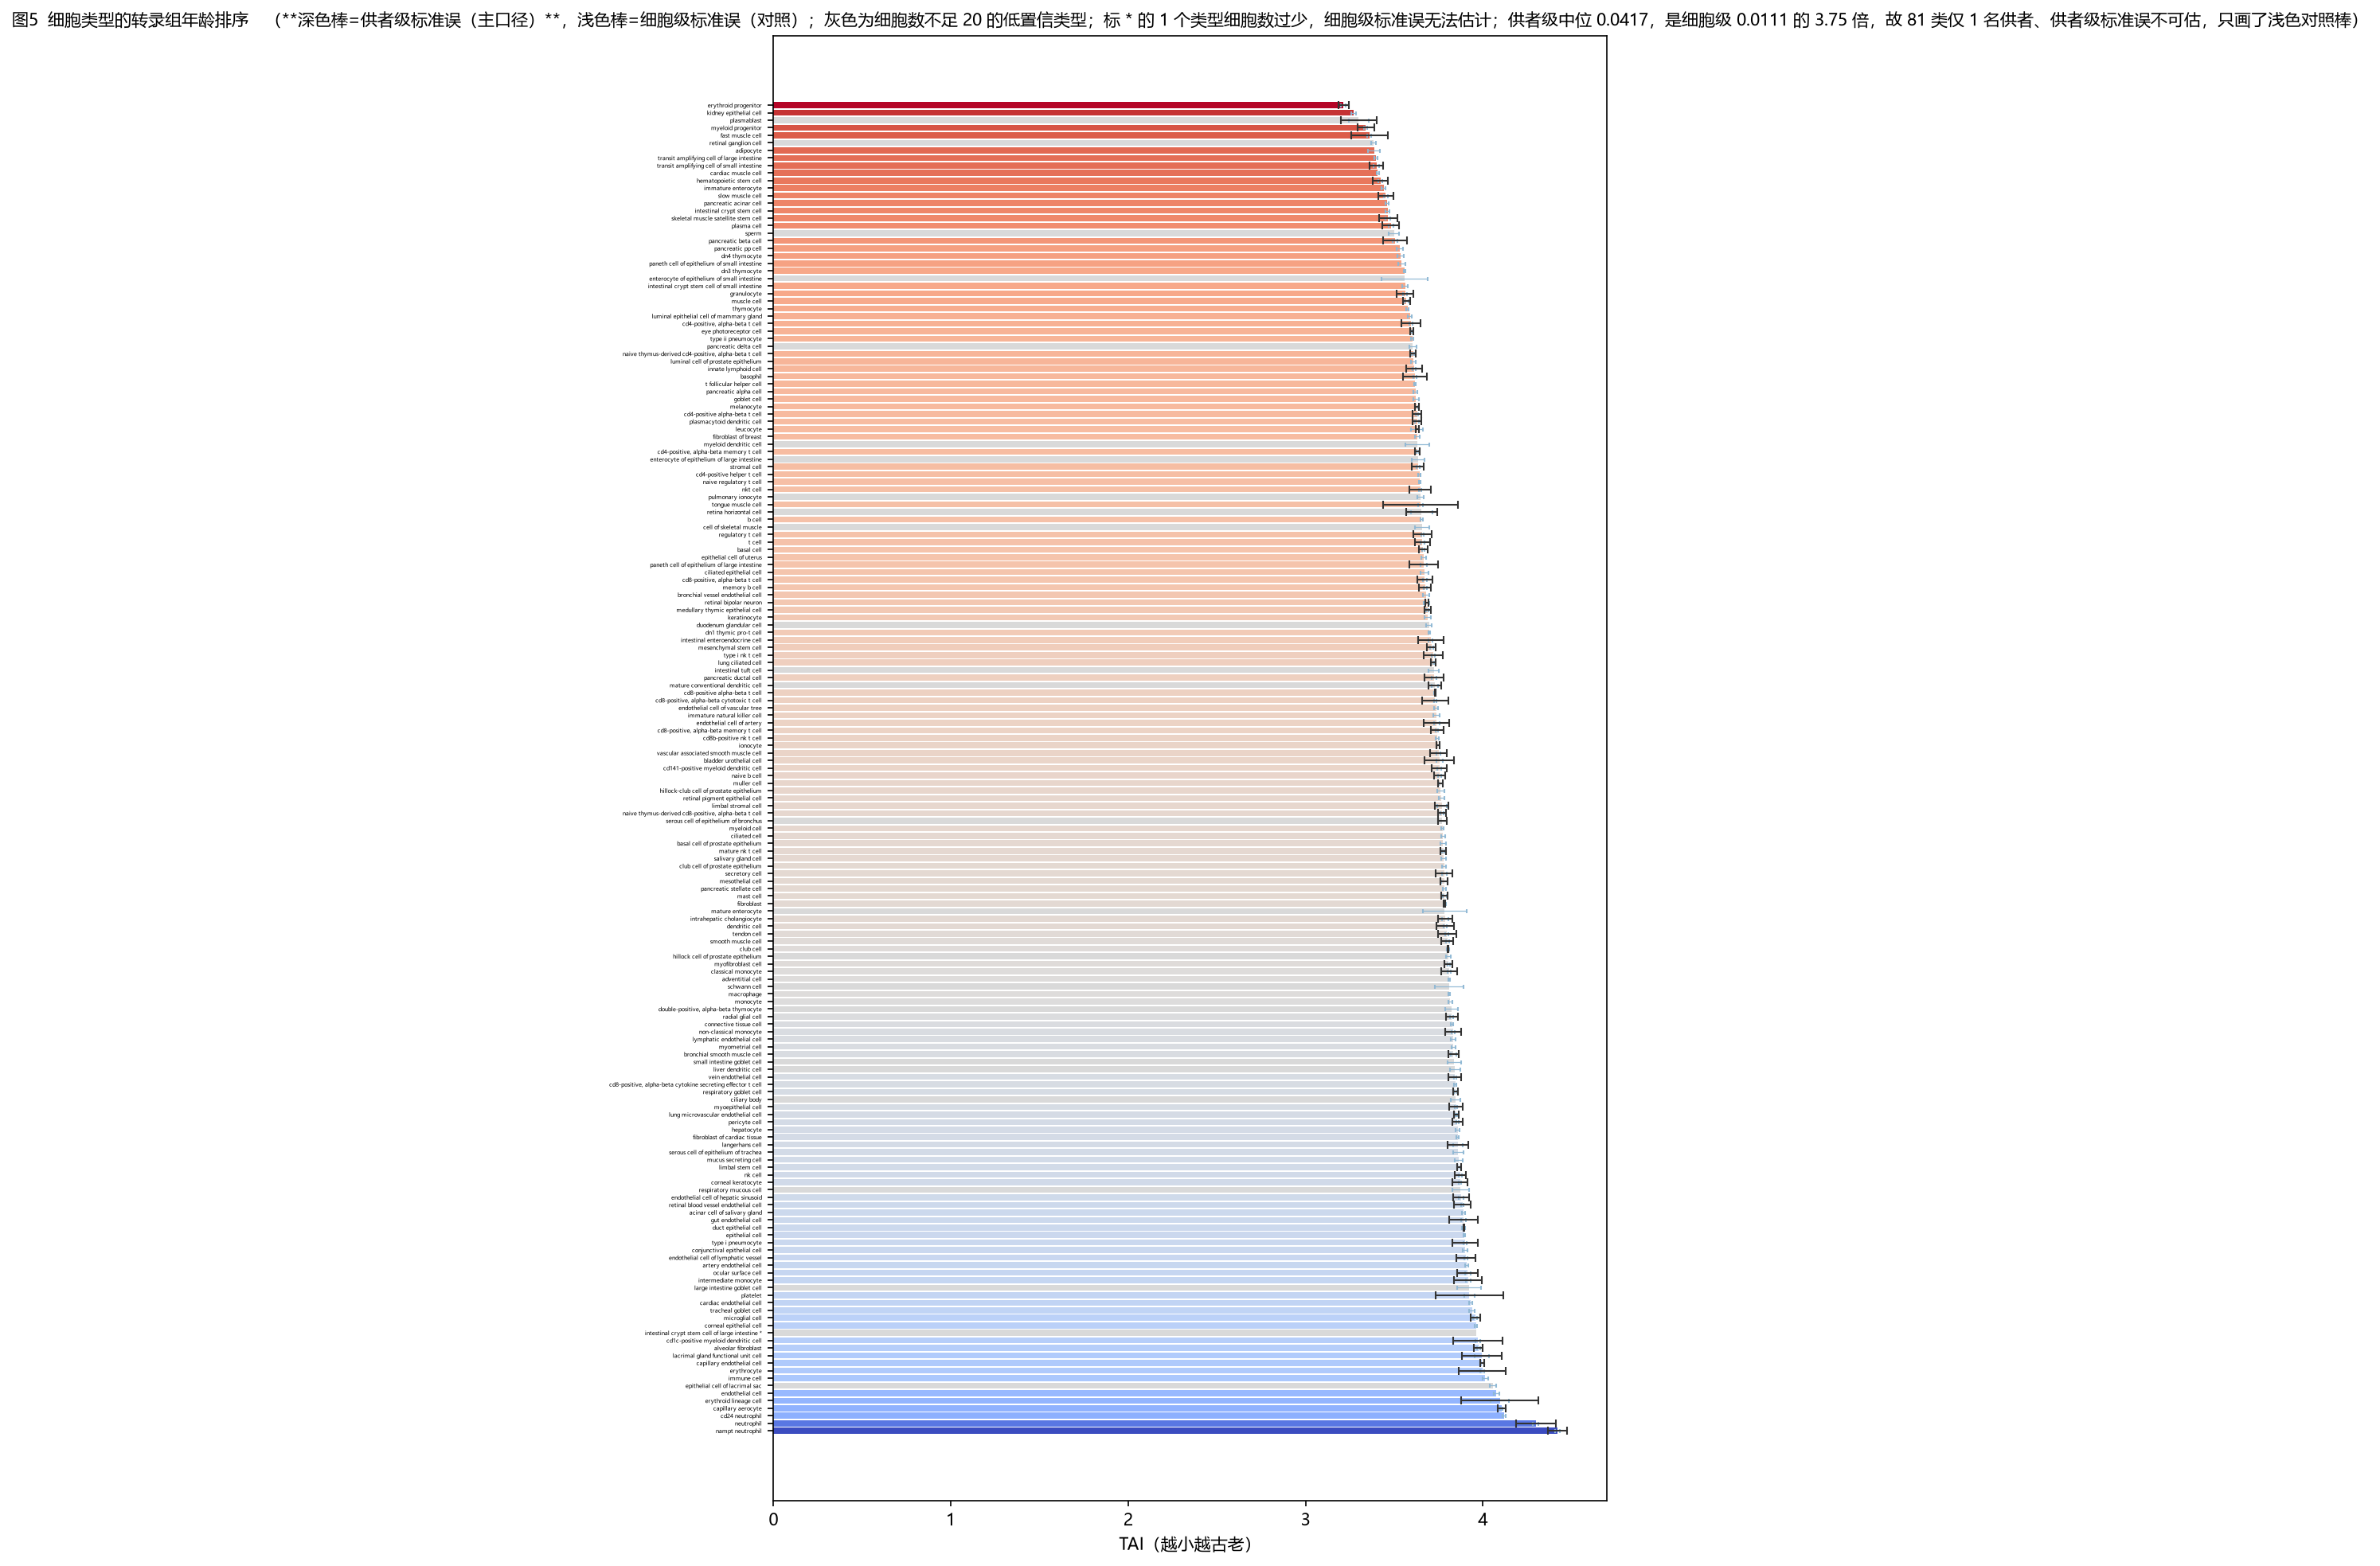
\includegraphics[width=\textwidth]{fig5_tai_rank.png}
  \caption{177 种细胞类型按 \tai{} 排序。误差棒同时给出两种口径：\textbf{深色粗棒 = 供者级标准误（主口径，与正文信号/噪声比同口径）}，浅色细棒 = 细胞级标准误（对照，直观显示按细胞计算会乐观多少）。灰色为细胞数 $< 20$ 的低置信类型；81 个单供者类型供者级不可估计，只画浅色棒。}
  \label{fig:rank}
\end{figure}

\subsection{年龄层的富集与耗竭}

经 BH 校正后，显著富集的年龄层为 \textbf{S1、S8、S9、S10、S11、S14}，显著耗竭为 \textbf{S2、S4}（图 \ref{fig:enrich}、表 \ref{tab:enrich}）。S10 的富集倍数最高（2.68 倍，$q = 1.4\times10^{-4}$），S11 次之（3.15 倍）。S2 与 S4 的耗竭最为显著（$q$ 分别为 $3.8\times10^{-16}$、$1.9\times10^{-5}$）。

\begin{table}[H]
  \centering
  \caption{各年龄层的富集倍数与 BH 校正后 $q$ 值（运行 A，全量）。完整 16 层见结果文件 \Code{age\_enrichment.tsv}}
  \label{tab:enrich}
  \begin{tabular}{lrrrlr}
    \toprule
    层 & 富集倍数 & $q_{\text{富集}}$ & 方向 & $q_{\text{耗竭}}$ & $q_{\text{耗竭}} < 0.05$ \\
    \midrule
    S1  & 1.35 & $4.5\times10^{-3}$  & 富集 & 1.00 & 否 \\
    S2  & 0.53 & 1.00               & \textbf{耗竭} & $3.8\times10^{-16}$ & \textbf{是} \\
    S4  & 0.43 & 1.00               & \textbf{耗竭} & $1.9\times10^{-5}$ & \textbf{是} \\
    S8  & 1.62 & $5.6\times10^{-7}$  & \textbf{富集} & 1.00 & 否 \\
    S9  & 1.81 & $2.7\times10^{-2}$  & \textbf{富集} & 1.00 & 否 \\
    S10 & 2.68 & $1.4\times10^{-4}$  & \textbf{富集} & 1.00 & 否 \\
    S11 & 3.15 & $8.8\times10^{-5}$  & \textbf{富集} & 1.00 & 否 \\
    S14 & 3.81 & $1.4\times10^{-2}$  & \textbf{富集} & 1.00 & 否 \\
    \bottomrule
  \end{tabular}
\end{table}

\begin{figure}[H]
  \centering
  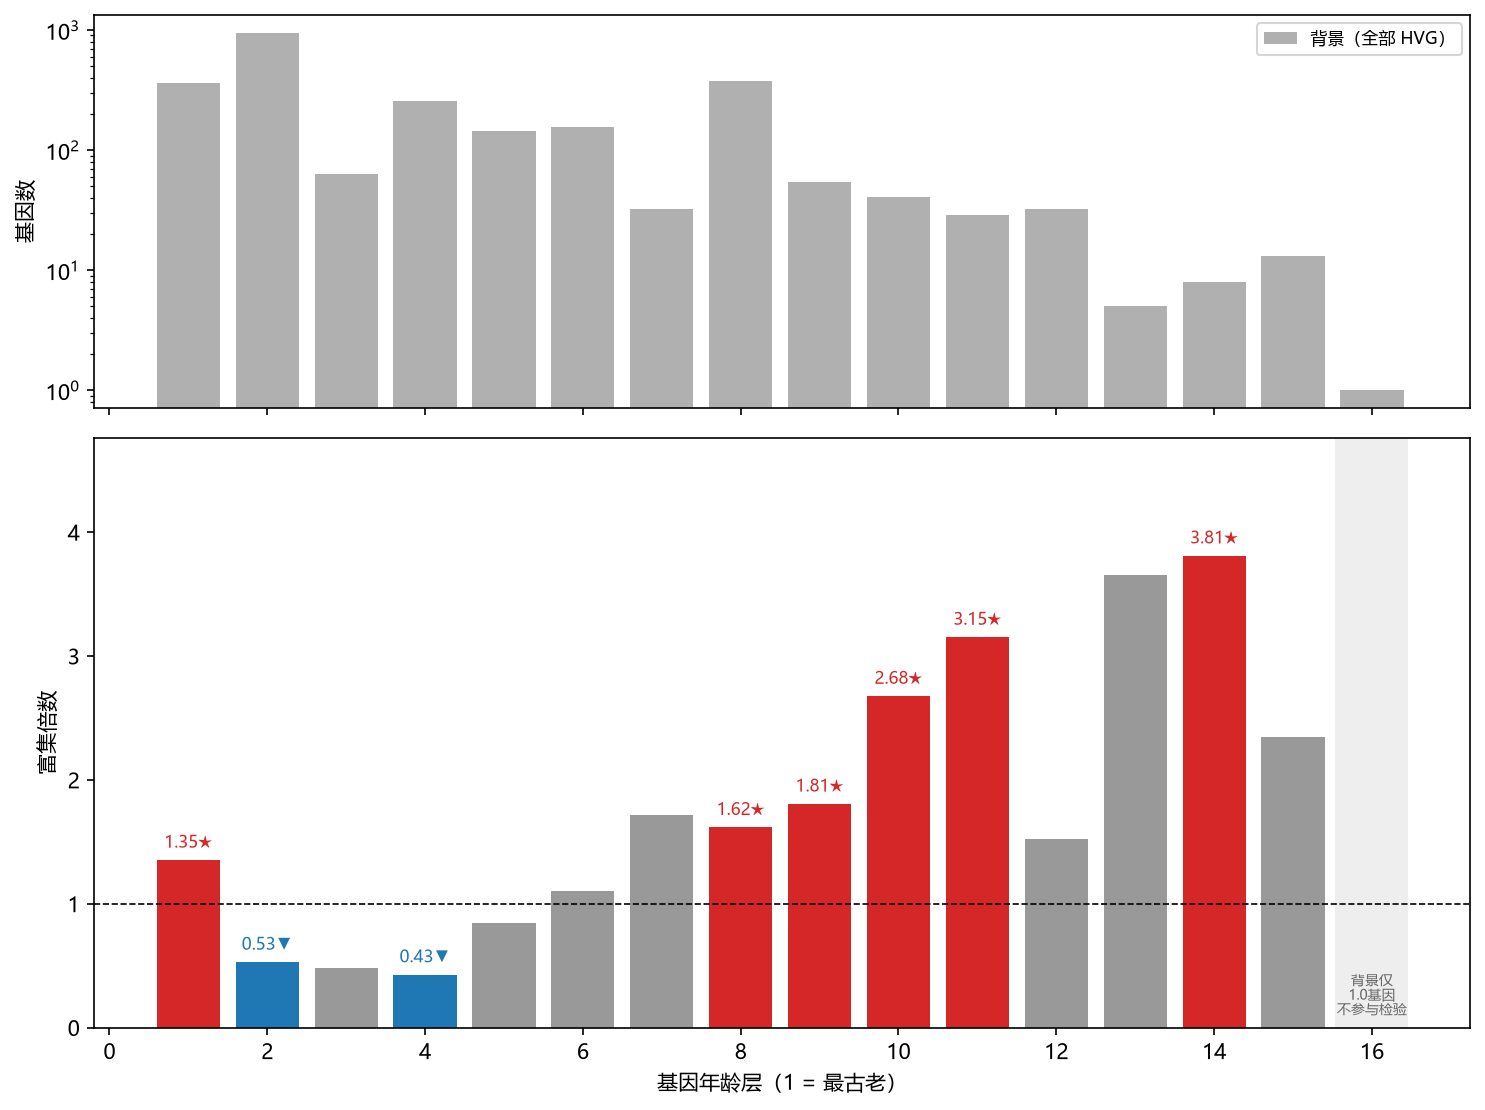
\includegraphics[width=\textwidth]{fig4_importance_age.png}
  \caption{上：各年龄层在背景高变基因中的基因数（对数轴）；下：Top 500 重要基因在各层的富集倍数。红色为 BH 校正后显著富集（$\star$），蓝色为显著耗竭（$\blacktriangledown$），灰底为背景基因过少、不参与检验的层。}
  \label{fig:enrich}
\end{figure}

\subsection{四重稳健性检验}

\begin{table}[H]
  \centering
  \caption{四重稳健性检验。检验 A = 全量；B = 共识度过滤（$\ge 0.8$）；C = 短蛋白剔除（$<100$ aa）；D = 长蛋白（$\ge 100$ aa）重算 \tai{}}
  \label{tab:robust}
  \begin{tabular}{lcccc}
    \toprule
    指标 & A（全量） & B（共识度） & C（短蛋白） & D（长蛋白） \\
    \midrule
    参与基因数 & 2{,}523 & 905 & 2{,}405 & 2{,}262 \\
    显著富集层 & S1,S8,S9,S10,S11,S14 & S8,S10 & S9,S10,S11,S14 & 见 \S\ref{sec:longprot} \\
    显著耗竭层 & S2,S4 & S2 & S2,S4 & --- \\
    \textbf{共同富集层} & \multicolumn{4}{l}{\textbf{S8、S10}（Jaccard = 0.333）} \\
    \textbf{共同耗竭层} & \multicolumn{4}{l}{\textbf{S2}} \\
    \textbf{方向冲突层数} & \multicolumn{4}{l}{\textbf{0}} \\
    准确率 & 0.215 & 0.180 & 0.213 & --- \\
    宏平均 F1 & 0.237 & 0.194 & 0.231 & --- \\
    \bottomrule
  \end{tabular}
\end{table}

前三次运行（A/B/C）的共同富集层为 \textbf{S8、S10}，共同耗竭层为 \textbf{S2}，\textbf{0 层出现方向冲突}。虽然每次运行的显著层集合并不完全相同，但\textbf{结论的方向在三种截然不同的数据口径下高度一致}。

\subsection{监督分类：准确率 0.215、天花板达成 36\%}

按供者划分的随机森林在测试集上准确率 \textbf{0.215}、宏平均 F1 \textbf{0.237}（显式指定标签集口径；默认口径为 0.164）。相对多数类基线（0.026）为 \textbf{8.26 倍}。

必须诚实披露的是\textbf{天花板问题}：177 种类型中有 28 种在训练集中完全未出现，占测试集细胞的 40.5\%，因此理论准确率上限仅为 \textbf{0.595}。本文的准确率 0.215 达到了天花板的 \textbf{36.1\%}。

\begin{figure}[H]
  \centering
  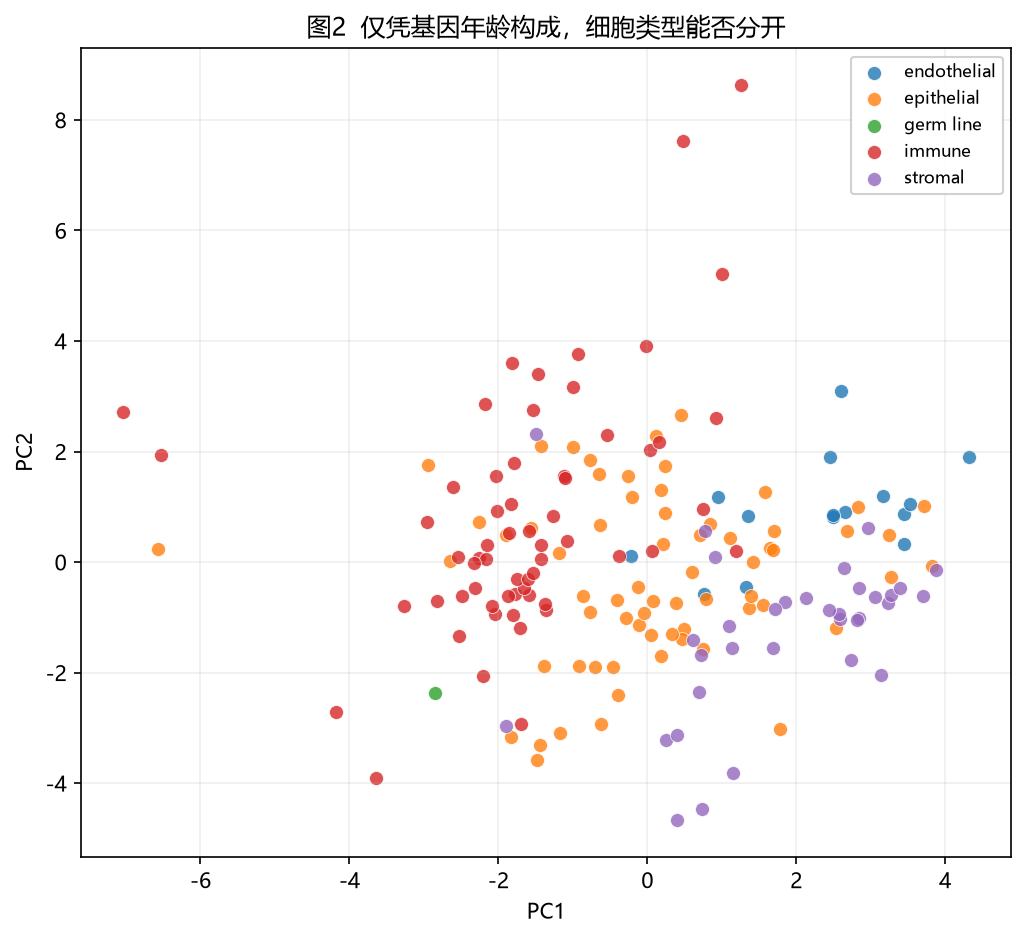
\includegraphics[width=0.88\textwidth]{fig2_pca.png}
  \caption{PCA 前两主成分散点，按 K-means 簇着色。}
  \label{fig:pca}
\end{figure}

\subsection{无监督结构与三条零假设基线}

PCA 前三主成分累计解释 \textbf{61.9\%} 方差（PC1 0.273、PC2 0.226、PC3 0.121），显著高于三条零假设基线：逐列置换 \textbf{27.05\%}、独立正态 \textbf{27.61\%}、Dirichlet 同秩 \textbf{29.03\%}，对应 $z = 47.0$ 与 $z = 48.3$。真实数据的秩为 15（16 层中一层冗余），参与比给出有效维度 \textbf{6.12}。

K-means（$k = 7$）的轮廓系数 0.235、ARI \textbf{0.211}，显著高于置换零假设（均值 $-0.0001 \pm 0.0104$，$z = 20.35$）。Ward 连接作为对照给出 ARI 0.170。低置信敏感性分析（$k = 5$）给出 ARI 0.159、轮廓 0.239、前三累计 63.4\%，结论方向不变。

\begin{figure}[H]
  \centering
  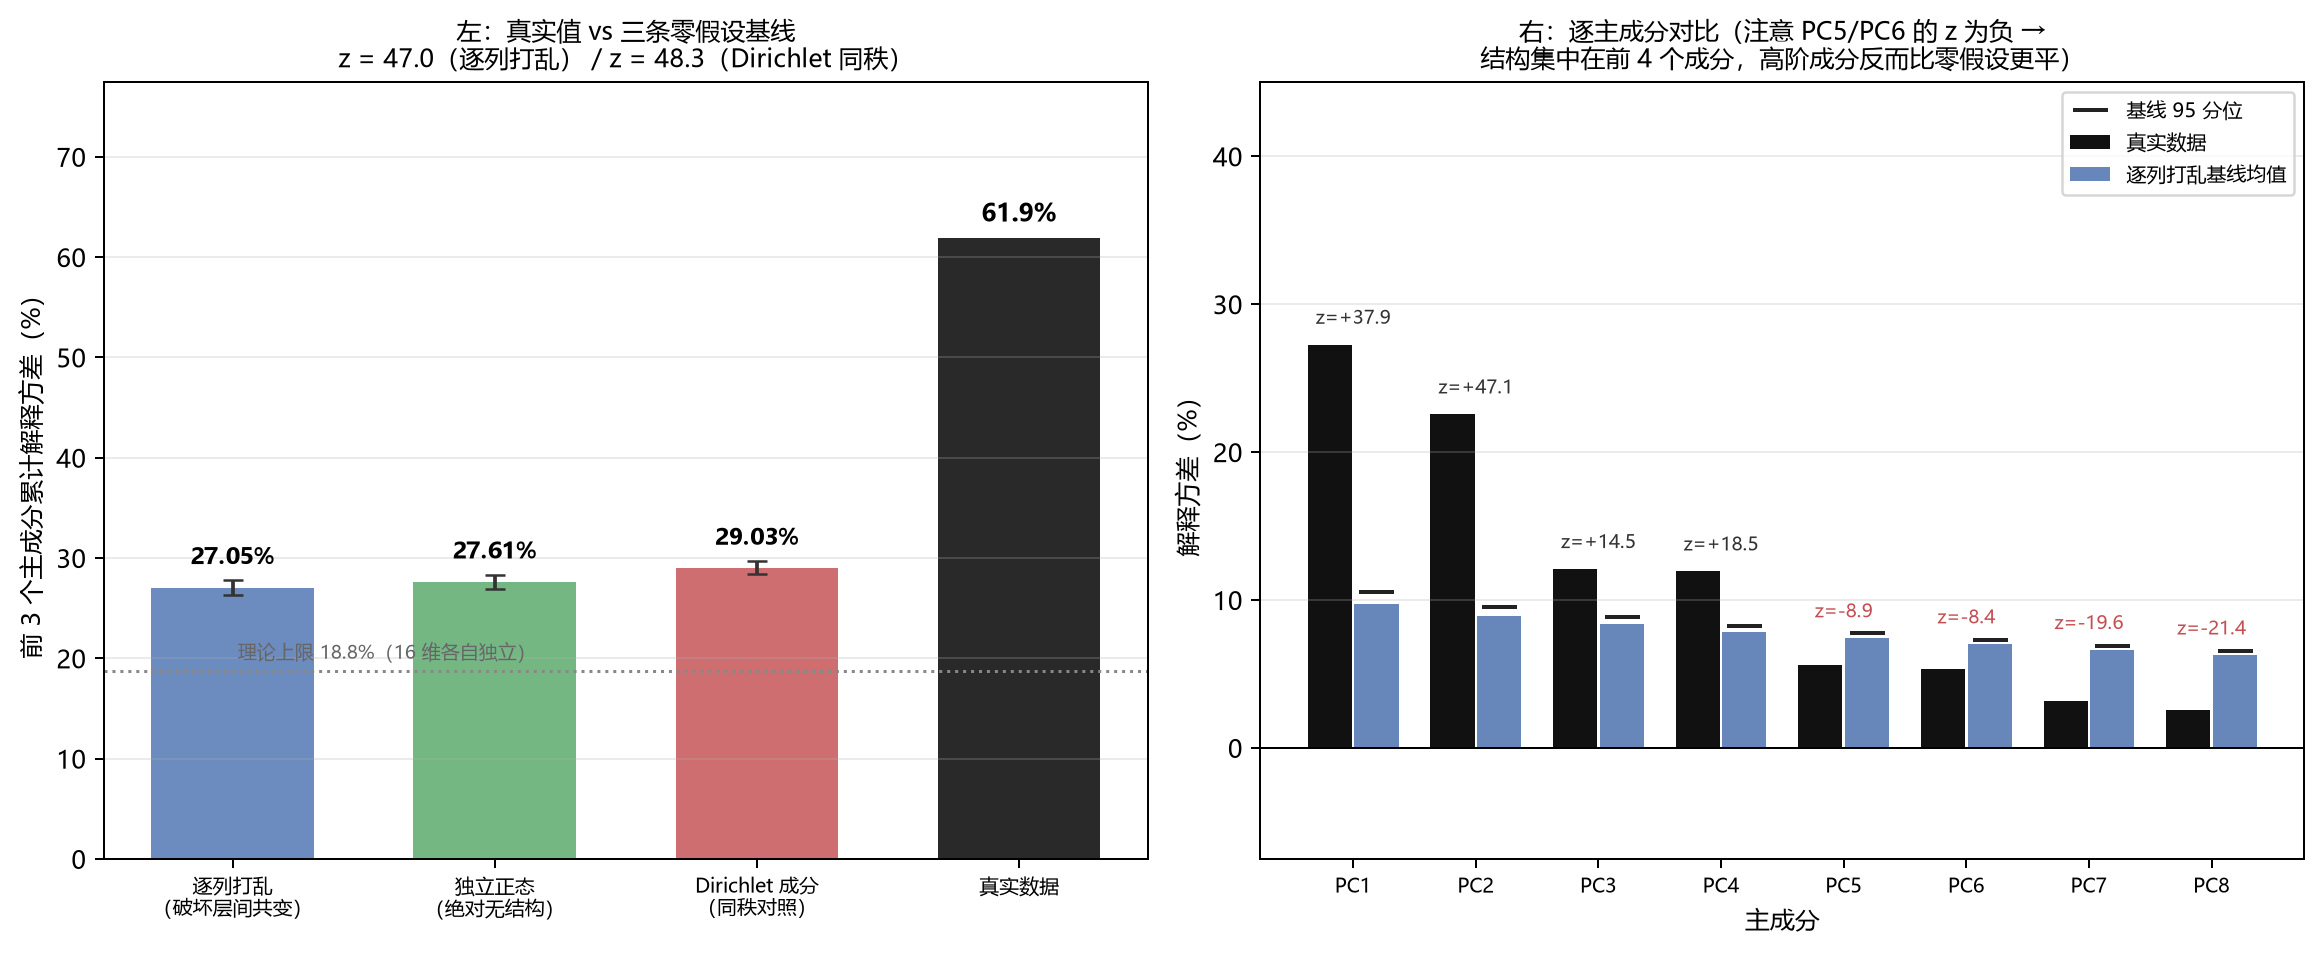
\includegraphics[width=\textwidth]{fig7_pca_null_baseline.png}
  \caption{\textbf{PCA 零假设诊断。}左：真实前三累计（61.9\%）vs 三条零假设基线（逐列置换 27.05\%、独立正态 27.61\%、Dirichlet 同秩 29.03\%），标注 $z = 47.0$ / $48.3$；右：逐主成分对比，PC5 之后 $z$ 值转负，说明结构集中在前 4 个成分。}
  \label{fig:pcanull}
\end{figure}

\subsection{检验 D：短基因偏倚的方向与大小}
\label{sec:longprot}

检验 C 证明了\textbf{结论不依赖短蛋白}，但批评者真正想问的是另一个问题：\textbf{如果只用长蛋白重算，绝对年龄会变成什么样？} 这是 Moyers 与 Zhang \citeyearpar{moyers2018} 建议的更彻底版本，也是本文此前唯一未完成的一环。

表 \ref{tab:longprot} 给出逐类型对照结果。关键发现有二：

\textbf{第一，偏倚表现为"系统性平移"，而非"随年龄梯度增强"。} 剔除短蛋白后\textbf{全部 177 种类型（100\%）}的 \tai{} 都下移，$\Delta\tai$ 均值 $-0.0572$、中位 $-0.0536$、标准差仅 0.0251；但下移幅度在古老类型（最古老 10 类均值 $-0.0663$）与年轻类型（最年轻 10 类均值 $-0.0725$）之间\textbf{几乎没有差别}，$\Delta\tai$ 与主口径 \tai{} 的秩相关仅 $-0.133$ 且不显著（$p = 0.079$）。

\begin{table}[H]
  \centering
  \caption{长蛋白版（$\ge 100$ aa）与主口径的对照}
  \label{tab:longprot}
  \begin{tabular}{lr}
    \toprule
    对照量 & 数值 \\
    \midrule
    Spearman $\rho$ & 0.9845 \\
    Kendall $\tau$ & 0.9186 \\
    $\Delta\tai$ 均值 / 中位 & $-0.0572$ / $-0.0536$ \\
    $|\Delta\tai|$ 中位 / 最大 & 0.0536 / 0.2523 \\
    同向平移的类型数 & 177 / 177（100\%） \\
    名次变动 / 最大位移 & 163 / 177，最大 79 位 \\
    Top10 重合 & 9 / 10 \\
    $\Delta\tai$ 的年龄梯度 $\rho$ & $-0.1326$（$p = 0.079$） \\
    \bottomrule
  \end{tabular}
\end{table}

这纠正了一个常见直觉：本文原以为"S15/S16 层以人类特异长链非编码 RNA 为主、可能造成对新近基因的低估"这一担忧会以年龄梯度的形式发生，但 TAI 这条证据表明\textbf{它并未以梯度的形式发生}——短蛋白确实集中在年轻层（见 \S\ref{sec:premise}），但把短蛋白整体剔除后，各类型被平移的幅度与它们的年龄高低无关。

\textbf{第二，绝对年龄受影响，但相对比较高度稳健。} 整体平移 0.057 约相当于跨类型标准差的 \textbf{31.6\%}；而排序 $\rho = 0.9845$、Top10 重合 9/10 说明"谁比谁更古老"这个相对结论几乎不动。

\begin{figure}[H]
  \centering
  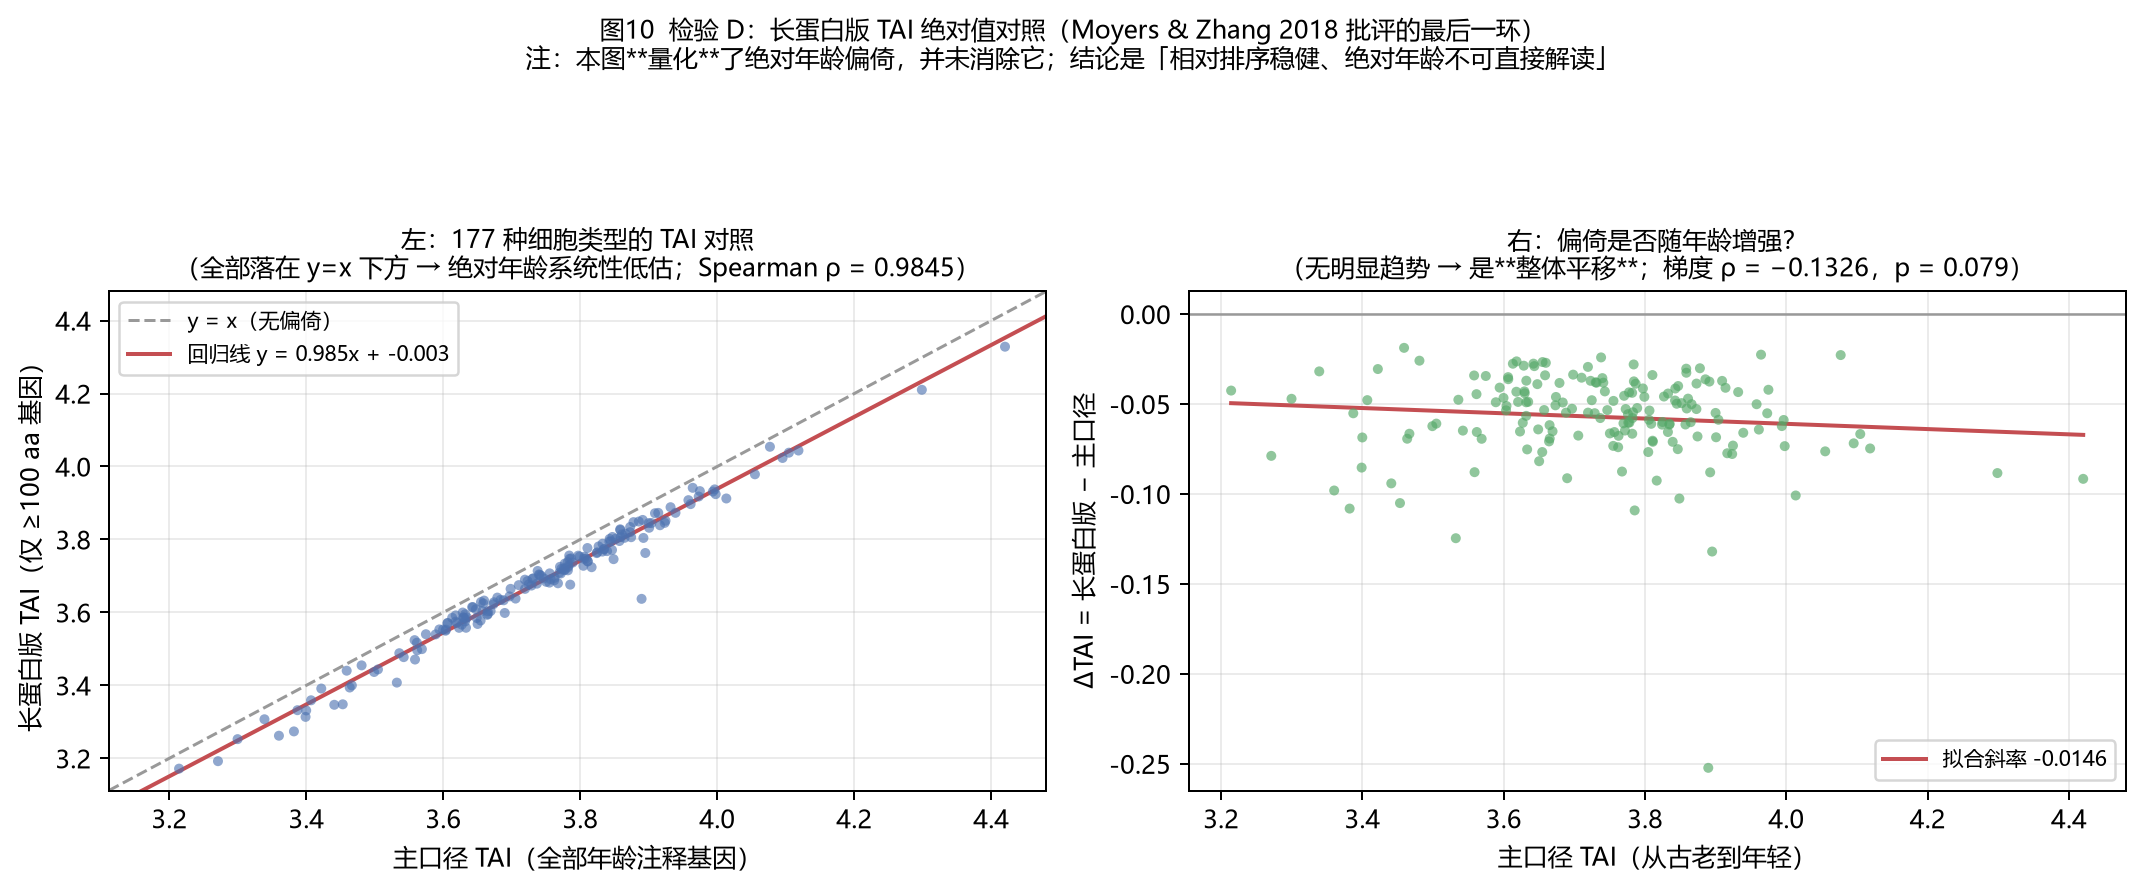
\includegraphics[width=\textwidth]{fig10_longprot_comparison.png}
  \caption{\textbf{检验 D：长蛋白版 \tai{} 绝对值对照。}左：主口径 \tai{} vs 长蛋白版 \tai{} 的 177 点散点与 $y=x$ 参考线，全部落在 $y=x$ 下方 → 绝对年龄被系统性低估（$\rho = 0.9845$）；右：$\Delta\tai$ 对主口径 \tai{} 的散点与拟合斜率（$-0.0146$），无明显年龄趋势 → 偏倚是\textbf{整体平移}而非随年龄梯度增强。}
  \label{fig:longprot}
\end{figure}

\subsection{检验 D 的前提：短蛋白确实集中在年轻层}
\label{sec:premise}

检验 D 的结果之所以有意义，前提是"短蛋白偏倚确实存在"。我们直接验证了这一前提：年龄层号与短蛋白（$< 100$ aa）占比的 Spearman $\rho = +0.871$，年轻层（S13--S16）短蛋白平均占比 \textbf{14.23\%}，是老层（S1--S4）的 \textbf{1.30\%} 的 \textbf{10.9 倍}；各层中位蛋白长度从 S1 的 454 aa 单调降至 S16 的 129 aa。

\begin{figure}[H]
  \centering
  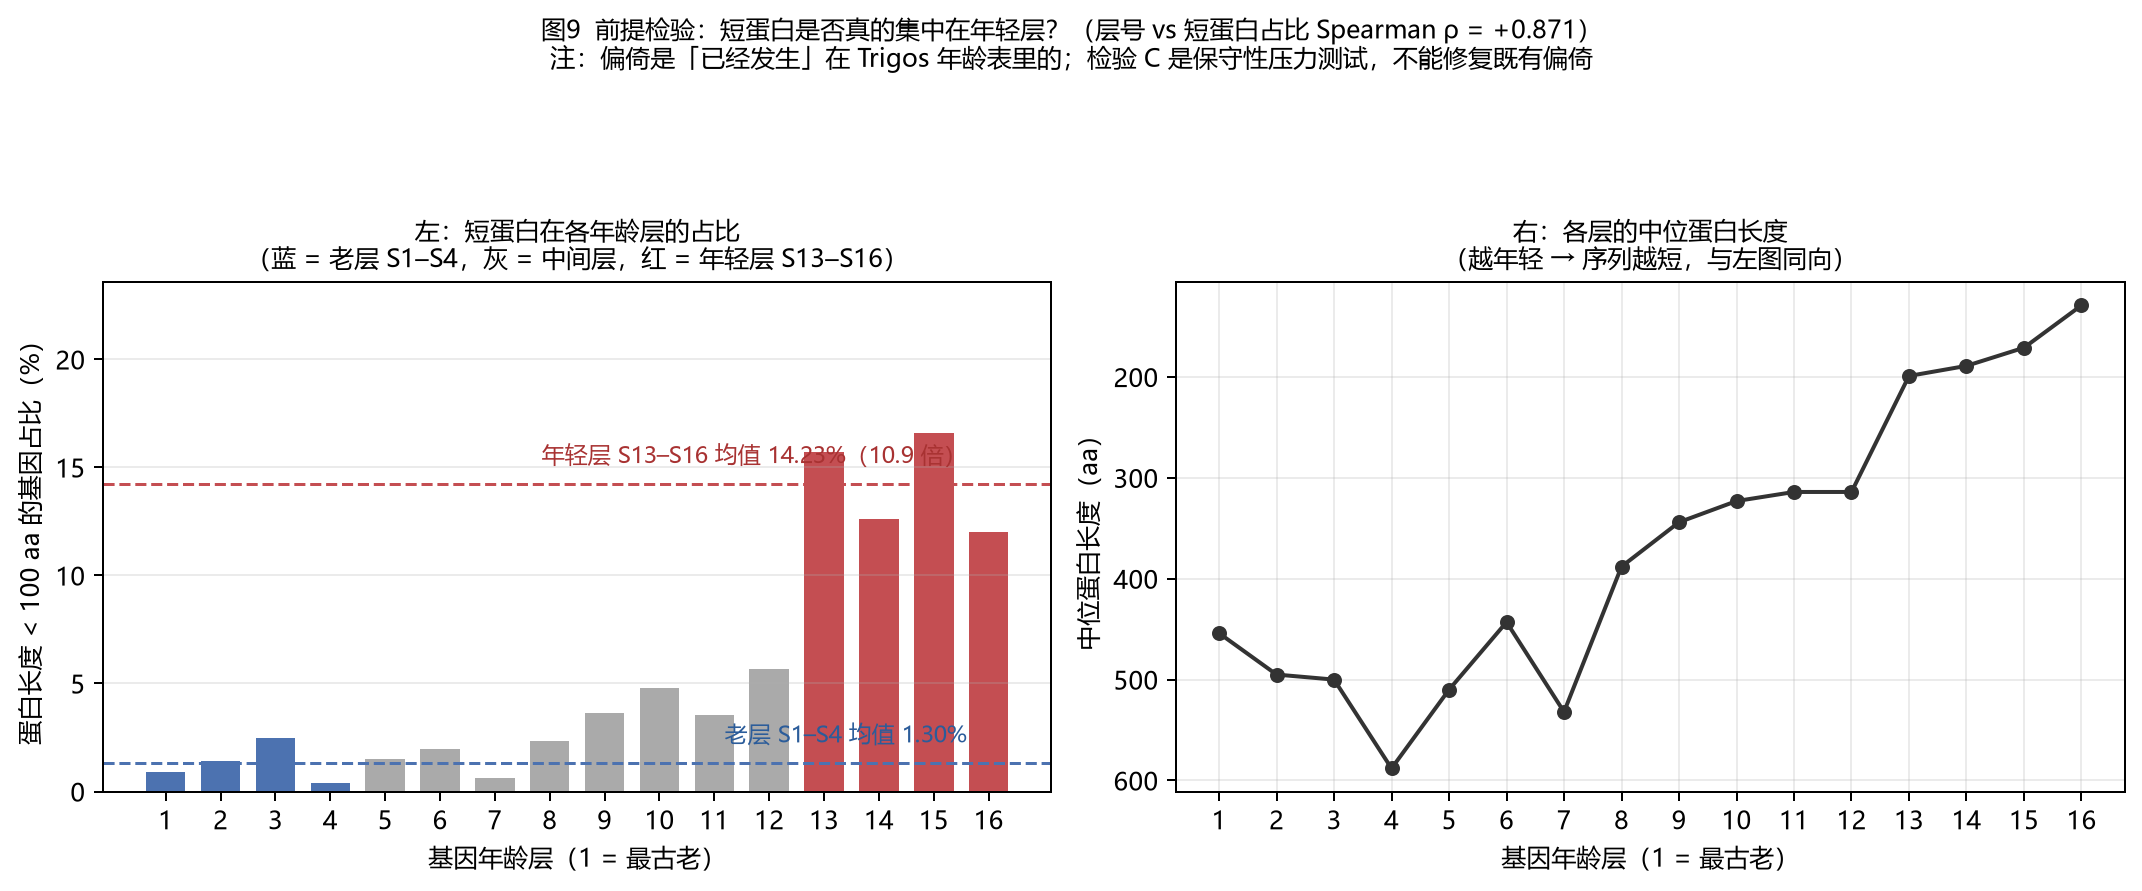
\includegraphics[width=\textwidth]{fig9_shortprot_premise.png}
  \caption{\textbf{短蛋白前提检验。}左：16 层的短蛋白（$< 100$ aa）占比柱状图，老层均值 1.30\% vs 年轻层均值 14.23\%（10.9 倍）；右：各层中位蛋白长度（454 aa $\to$ 129 aa 单调下降）。}
  \label{fig:premise}
\end{figure}

\section{讨论}

\subsection{主要发现与解读}

本文给出了一个\textbf{可复现、数据驱动}的框架，把"细胞类型有多古老"从定性描述变为定量测量。三个层次的结论：

\textbf{存在真实的年龄梯度。} 177 种细胞类型的 \tai{} 连续分布在 3.214--4.420 之间，跨类型标准差 0.181，且该结构在四条零假设基线之上（$z = 47.0$），在四重稳健性检验下方向零冲突。

\textbf{梯度是"配比"而非"有无"。} 即使最年轻的类型也保留大量 S1--S4 的古老基因；细胞类型之间的差异在于各年龄层的\textbf{比例配置}，而非某类细胞缺少古老成分。这提示细胞类型的演化更像是\textbf{同一套古老底层上的重新加权}，而非从零开始的模块化拼装。

\textbf{绝对年龄不可直接解读，相对比较才是可靠产出。} 供者级信号/噪声比仅 4.3 倍，且检验 D 证明 phylostratigraphy 的绝对年龄带有约 0.057（占跨类型 SD 31.6\%）的系统性偏差。因此本文\textbf{不对任何基因或类型的绝对年龄下断言}，全部结论建立在跨类型的相对比较上，而相对比较对这一偏差稳健。

\subsection{与既有工作的关系}

本文不与 Trigos \citeyearpar{trigos2017} 或 Domazet-Lošo \citeyearpar{domazetloso2017} 竞争基因年龄估计的精度——那需要更多的物种参照与更精细的算法。本文做的是把已有的年龄表\textbf{投射到单细胞类型层面}，并首次把 phylostratigraphy 的已知方法学偏差在细胞类型粒度上\textbf{定量}出来。

与组织层面的转录组年龄工作 \citeyearpar{lu2017} 相比，本文的粒度更细，且额外处理了两个在组织层面不会出现的问题：供者级伪重复（组织样本的重复来自个体，细胞级的重复来自供者内个体）与组成数据的秩亏。

\subsection{方法学教训}
\label{sec:pitfalls}

本文在开发过程中实际发现并修复了七类"脚本不报错但数字错误"的缺陷。它们都属于\textbf{静默失败}：代码正常退出、输出格式正常，但结论是错的。这类缺陷只能靠\textbf{断言式数字终审}来拦截。

\begin{enumerate}[label=\arabic*.]
  \item \textbf{双单尾的右尾退化}：超几何检验的右尾 $p \approx 1$ 并不意味着"无证据富集"，而是意味着"有耗竭证据"；耗竭方向必须用左尾 $\mathrm{cdf}(k)$，否则耗竭层会被漏报。
  \item \textbf{派生列泄漏}：把目标列算出的统计量再作为特征喂回模型，会得到虚高到 0.99 的准确率。
  \item \textbf{\texttt{numpy.argmax} 遇 NaN 返回 NaN 下标}：取最大值的标签必须用 \texttt{df.dropna().idxmax()}。
  \item \textbf{PCA 零假设的置换对象错误}：置换样本行不改变特征协方差，零假设分布退化为观测值本身（基线 = 真实值、$z = 0$）且不报任何错。
  \item \textbf{Spearman 的同义反复}：\texttt{scipy.spearmanr} 对 pandas Series 按\textbf{位置}取值，两列各自升序时位置秩相关\textbf{恒等于 $+1$}（500/500 复现）。必须先按索引对齐再算；修正后 $\rho = 0.9883$。
  \item \textbf{宏平均 F1 的幽灵类}：默认标签集合取 $y_{\text{true}} \cup y_{\text{pred}}$，会被预测出的测试集未见类稀释（0.164 $\to$ 0.237）。必须显式指定。
  \item \textbf{共识度字段的语义误读}：\texttt{NumDBsContributing} 是分母不是支持数，按它过滤方向是反的。
\end{enumerate}

此外还有两处结构性陷阱值得强调：\textbf{组成数据的秩亏}（占比行和恒为 1 → 协方差秩亏到 $d-1$，零假设必须同秩，否则基线被秩亏推高）；以及\textbf{图与正文的统计口径必须一致}（正文改用保守的供者级口径而图仍画乐观的细胞级，等于暗示"图比文可信"）。

\subsection{局限}

\begin{enumerate}[label=\arabic*.]
  \item \textbf{单一数据源}：仅使用 Tabula Sapiens 1.0，缺少跨队列验证。
  \item \textbf{单细胞异质性被聚合掩盖}：类型级聚合丢失了同一类型内的年龄构成异质性（这里用年龄构成的 Shannon 多样性作为代理指标）。
  \item \textbf{年龄表分辨率固定}：16 层是粒度上限，无法区分同层内的精细年龄差异。
  \item \textbf{未做跨组织、跨发育阶段的系统比较}：如需回答"同一谱系在发育过程中是否年轻化"，需要引入时间序列数据。
  \item \textbf{分类任务的绝对难度高}：宏平均 F1 0.237 反映的是 \textbf{177 分类别任务的真实困难程度}（天花板 0.595），而非模型调参不足。
  \item \textbf{绝对年龄的偏倚已被量化，但未被消除}：检验 D 给出的是"偏倚有多大"的估计，不是修正。
\end{enumerate}

\section{结论}

本文把系统发育地层学从基因层面推广到\textbf{细胞类型层面}，得到三点结论：

\begin{enumerate}[label=\arabic*.]
  \item 人体 177 种细胞类型存在\textbf{清晰、连续、可复现的转录组年龄梯度}（\tai{} 3.214--4.420），且该梯度在四重稳健性检验下方向零冲突、在四条零假设基线之上显著（$z = 47.0$）。
  \item 细胞类型之间的差异体现为\textbf{年龄层的配比}，而非"是否含有古老基因"——所有类型都保留了古老的底层结构。
  \item phylostratigraphy 的绝对年龄带有\textbf{已量化的系统性偏倚}（长蛋白重算使全部类型同向平移 0.057，约占跨类型 SD 的 31.6\%，且与年龄高低无关）。因此\textbf{相对排序是可靠的产出，绝对年龄不可直接断言}。
\end{enumerate}

方法学上，本文的可复现性保障是\textbf{自动数字终审}：论文与报告中的每个关键数字都是一条与输出文件比对的断言（239 项），任何不一致都会让流水线以非零码退出。这套机制在开发中拦下了七类静默失败。

\textbf{数据与代码可得性}：Tabula Sapiens 1.0 \citeyearpar{conservation2020}；年龄表来自 Trigos et al. 2017 \citeyearpar{trigos2017} 与 Liebeskind et al. 2016 \citeyearpar{liebeskind2016}；蛋白长度来自 UniProt。全部分析代码、结果表与图以开源仓库发布。

\section*{致谢}
感谢 Tabula Sapiens Consortium \citeyearpar{conservation2020} 与 CELLxGENE 平台提供公开数据。

\bibliographystyle{plainnat}
\bibliography{references}

\appendix
\section{算法流程}

本项目的完整分析流水线包含以下 12 个步骤：

\begin{enumerate}[label=\textbf{S\arabic*.}]
  \item \textbf{远程探测}：读取 HDF5 对象头，确认 dataset 分块与维度（\Code{90\_远程探测h5ad.py}）。
  \item \textbf{远程切片}：按 chunk 粒度规划 HTTP Range 请求，提取 28{,}017 个细胞的稀疏计数矩阵（\Code{92\_远程切片.py}）。
  \item \textbf{年龄表构建}：双来源交叉验证，输出 \Code{gene\_age.tsv}，含层号、共识度与低置信标记（\Code{02\_构建年龄表.py}）。
  \item \textbf{数据体检}：检查矩阵稀疏度、基因数、线粒体比例等，记录于体检日志（\Code{01\_检查数据.py}）。
  \item \textbf{核心计算}：QC、类型级聚合、逐细胞 \tai{}、类型级 \tai{}、供者级标准误（\Code{03\_细胞类型年龄谱.py}）。
  \item \textbf{无监督分析}：PCA + K-means + ARI + 置换零假设 + 低置信敏感性分析（\Code{04\_无监督分析.py}）。
  \item \textbf{监督分析}：按供者划分的随机森林 + BH 校正的超几何富集检验（\Code{05\_监督分析.py}）。
  \item \textbf{稳健性对比}：三次运行逐层对照 + 短蛋白前提检验（\Code{06\_稳健性对比.py}）。
  \item \textbf{主成分诊断}：三条零假设基线、载荷结构、参与比（\Code{08\_主成分诊断.py}）。
  \item \textbf{长蛋白对照}：重算 \tai{} 绝对值并逐类型比较（\Code{94\_长蛋白对照.py}）。
  \item \textbf{画图与网页}：十张图与交互式网页（\Code{06\_画图.py}、\Code{07\_做网页.py}）。
  \item \textbf{数字终审}：239 项断言与输出文件比对（\Code{07\_终审核对.py}）。
\end{enumerate}

\section{关键参数}

\begin{table}[H]
  \centering
  \caption{关键参数一览}
  \label{tab:params}
  \begin{tabular}{ll}
    \toprule
    参数 & 取值 \\
    \midrule
    年龄层数（Trigos 2017） & 16 \\
    QC 后细胞数 / 细胞类型数 & 22{,}195 / 177 \\
    富集检验背景基因数 & 2,523（测试 C 下为 2,405） \\
    显著性阈值（BH 校正后） & $q < 0.05$ \\
    随机森林特征数（运行 A） & 3,000（运行 B：905；运行 C：2,405） \\
    训练 / 测试供者数 & 11 / 4 \\
    K-means 簇数 & 7（敏感性分析：5） \\
    短蛋白阈值 & $< 100$ aa（检验 C 剔除） \\
    长蛋白重算阈值（检验 D） & $\ge 100$ aa，查不到长度的基因\textbf{保留} \\
    PCA 零假设置换次数 & 1,000 \\
    \bottomrule
  \end{tabular}
\end{table}

\section{补充图表}

\begin{figure}[H]
  \centering
  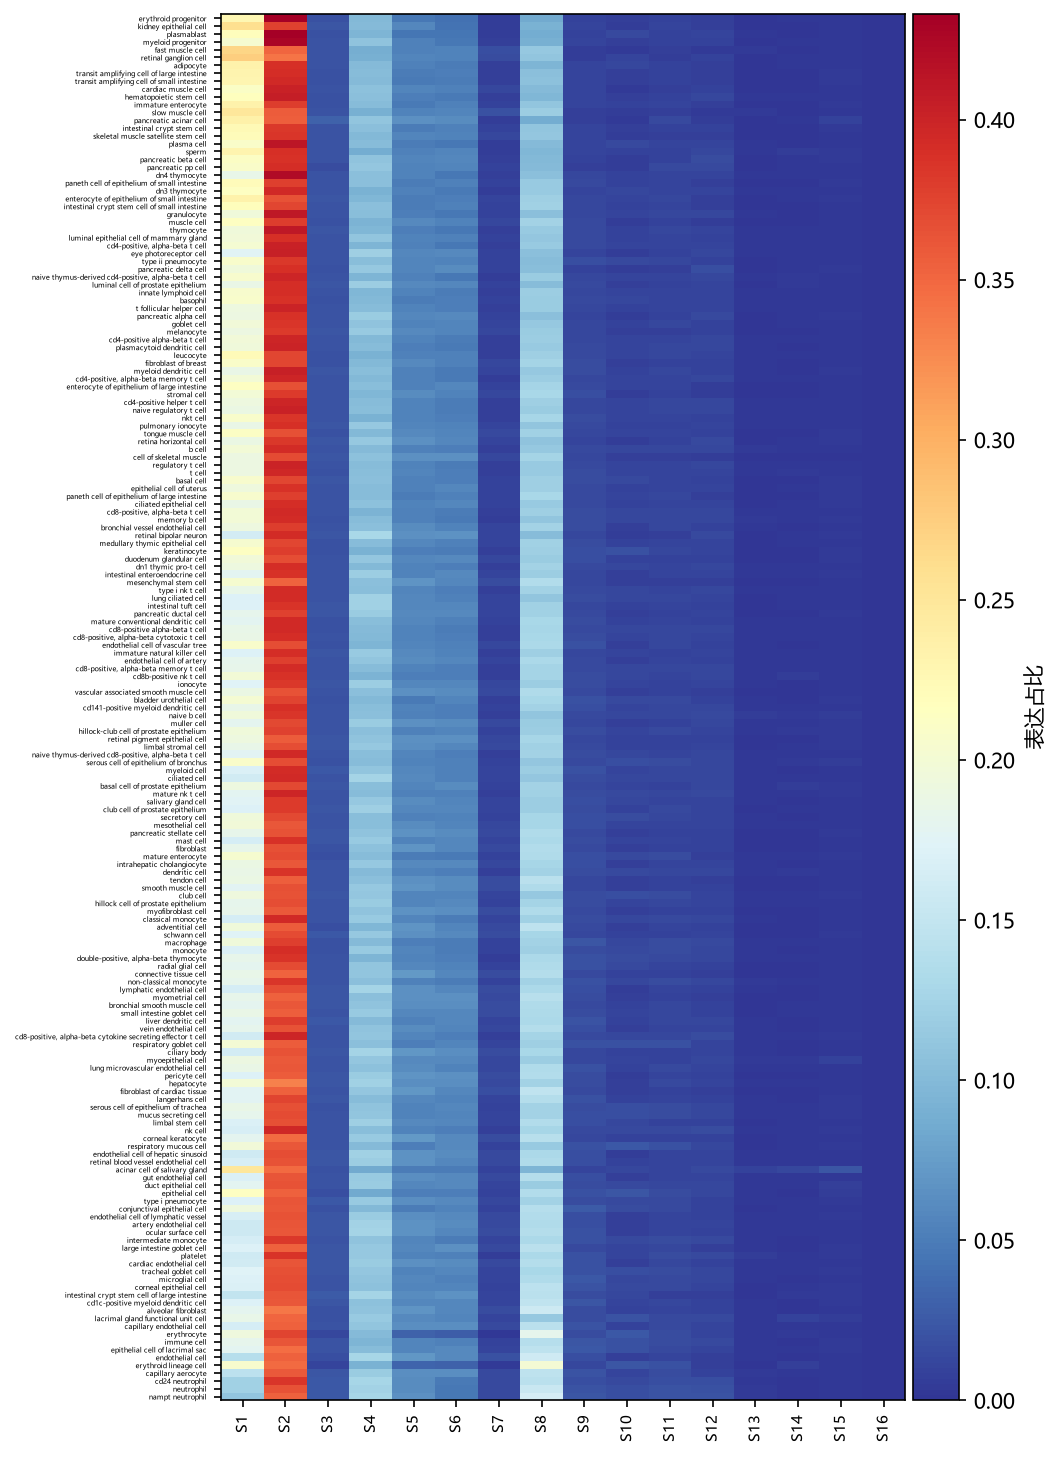
\includegraphics[width=0.95\textwidth]{fig3_heatmap.png}
  \caption{行 = 细胞类型（按 \tai{} 排序），列 = 16 个年龄层，颜色 = 表达占比。图注标注红端对应古老层。}
  \label{fig:heatmap}
\end{figure}

\begin{figure}[H]
  \centering
  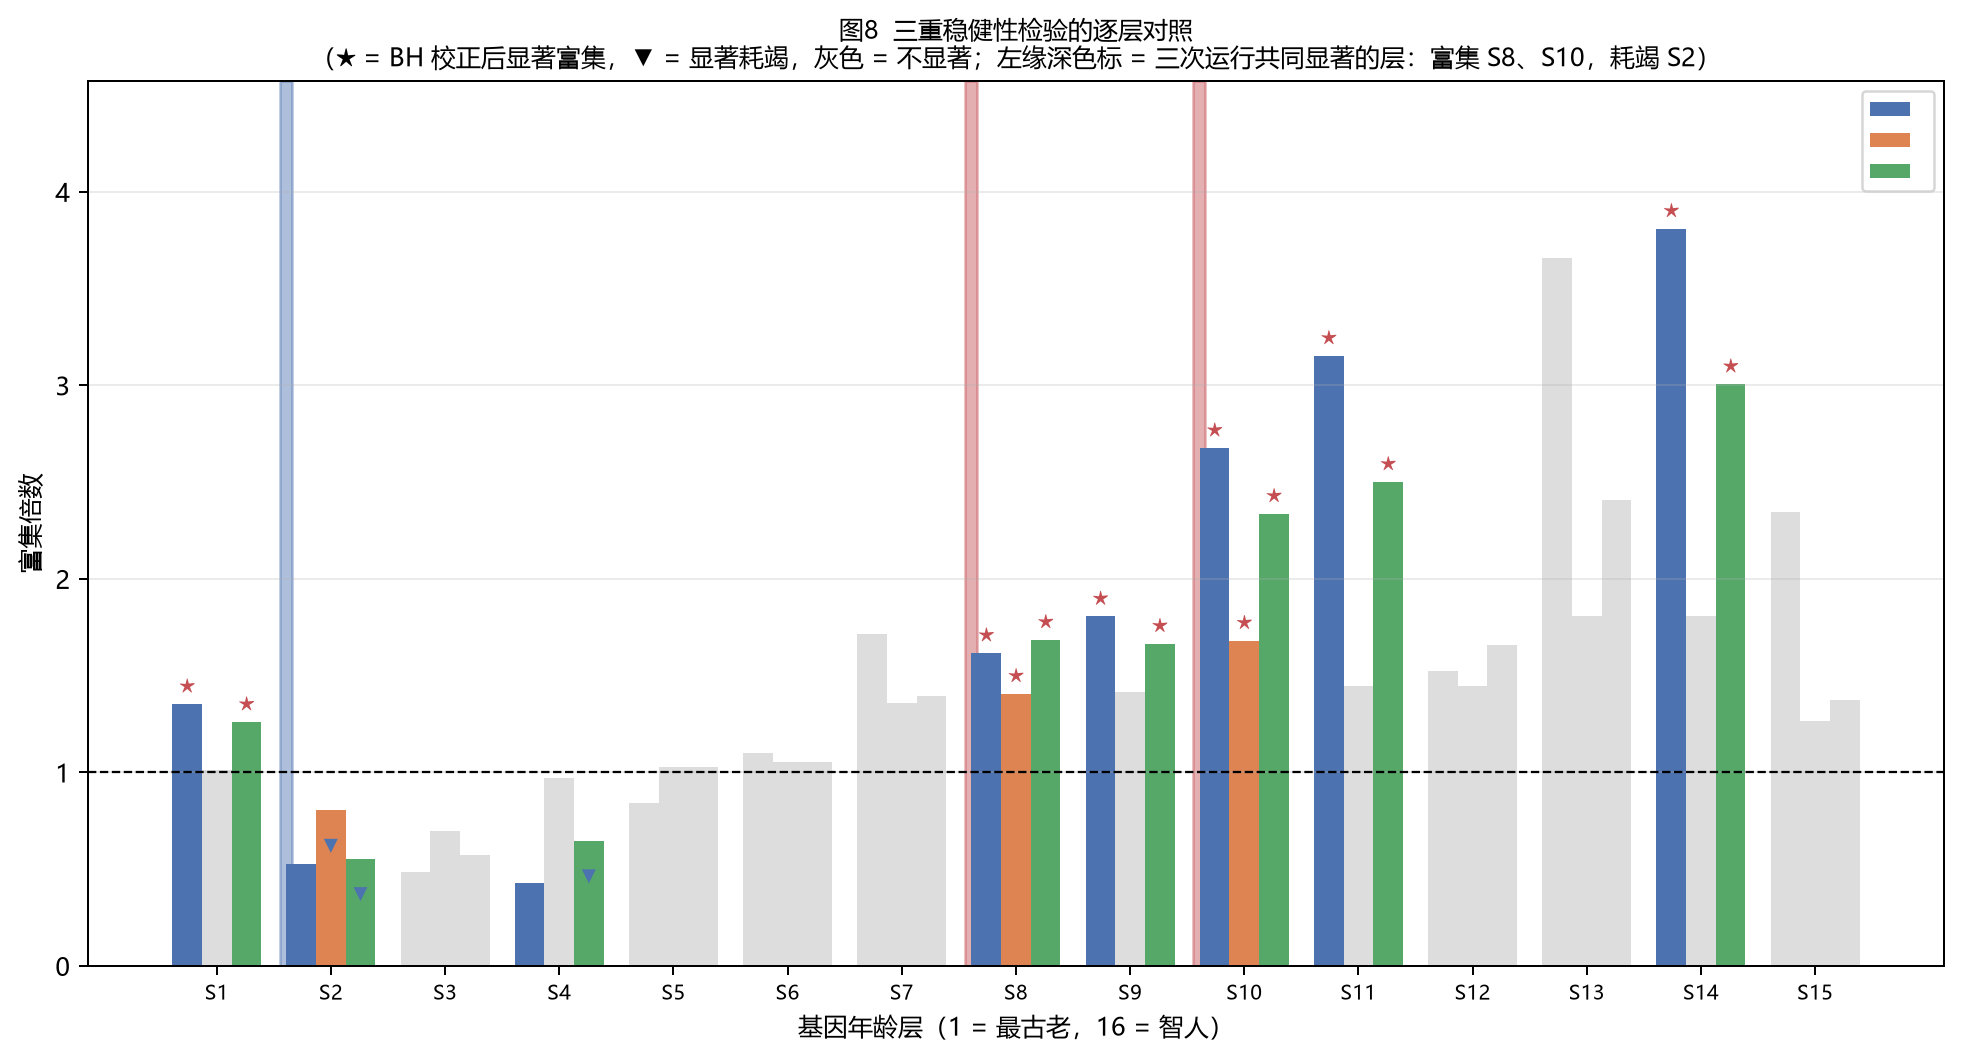
\includegraphics[width=\textwidth]{fig8_robustness_layers.png}
  \caption{\textbf{三重稳健性逐层对照。}横轴 S1--S15，每层三条柱（A 全量 / B 共识度过滤 / C 短蛋白剔除）的富集倍数；$\star$ / $\blacktriangledown$ = BH 校正后显著，左缘深色标 = 三次共同显著层（富集 S8、S10；耗竭 S2）。}
  \label{fig:rob}
\end{figure}

\begin{figure}[H]
  \centering
  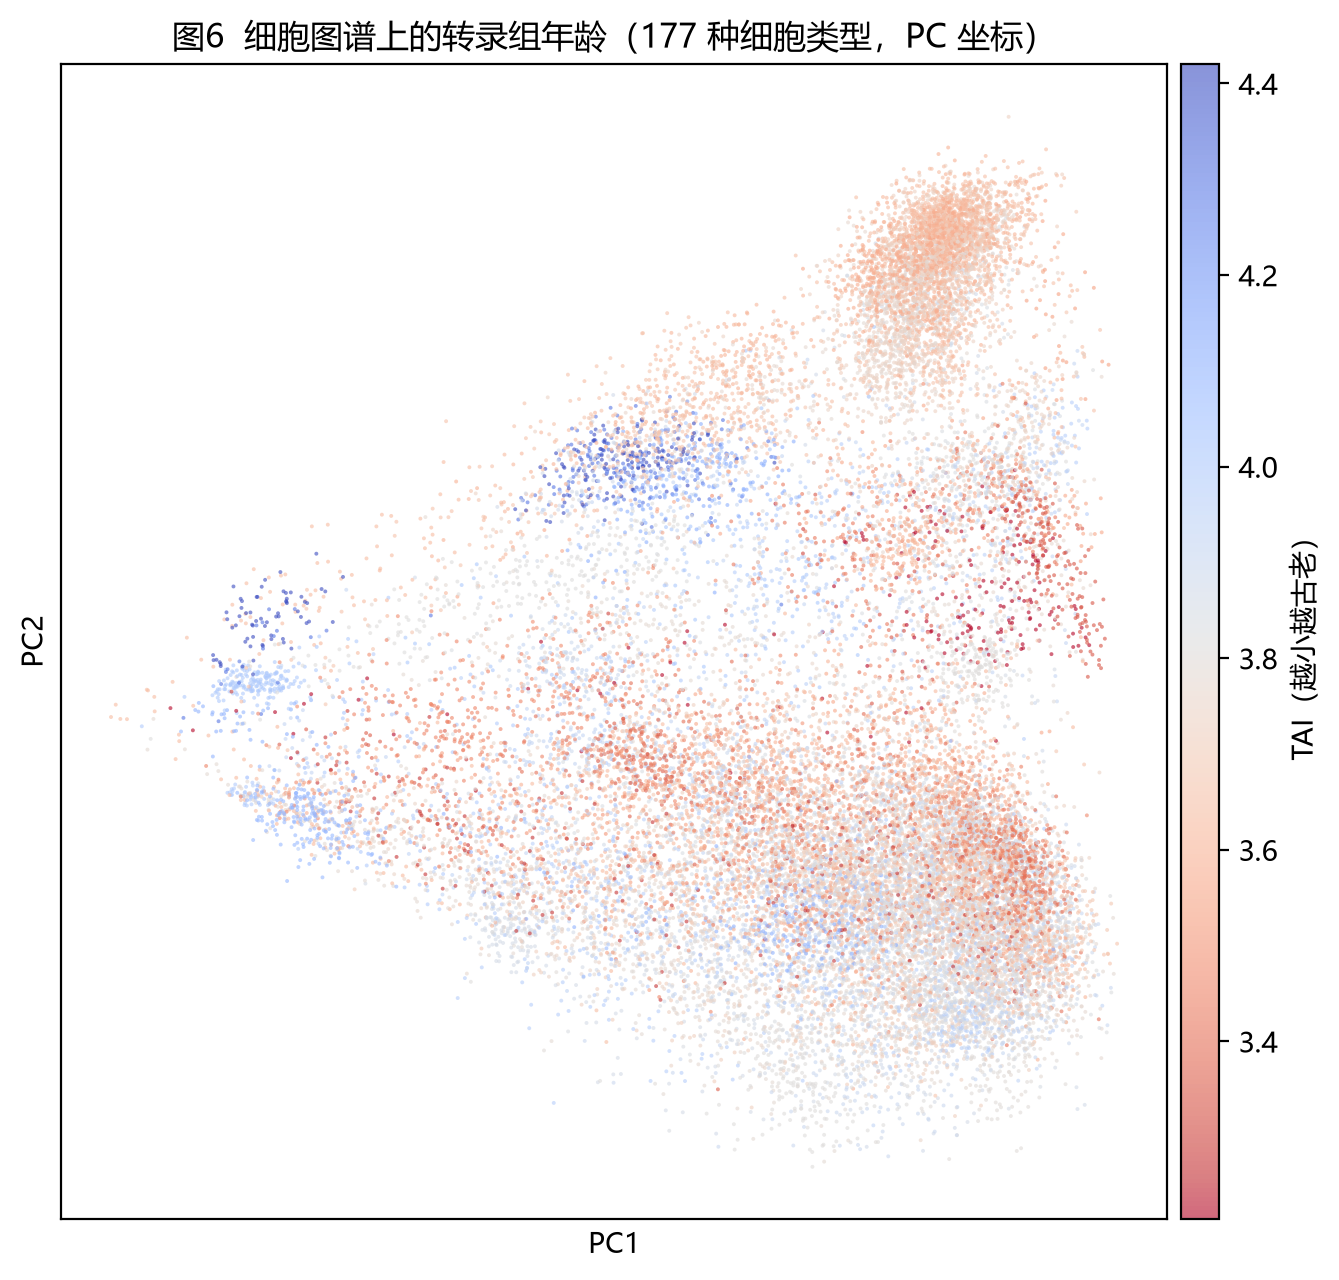
\includegraphics[width=0.9\textwidth]{fig6_umap_tai.png}
  \caption{细胞的 PC1/PC2 投影，按所属细胞类型的 \tai{} 着色（切片源用稀疏 SVD 代替 UMAP）。}
  \label{fig:umap}
\end{figure}

\end{document}
